\documentclass{article}
\usepackage[12pt]{extsizes}
\usepackage[utf8]{inputenc}
\usepackage[T1,T2A]{fontenc}
\usepackage[english,russian]{babel}
\usepackage{setspace,amsmath}
\usepackage{enumitem}
\usepackage{etoolbox}
\usepackage[usenames, dvipsnames]{color}
\usepackage[left=30mm, top=20mm, right=20mm, bottom=20mm, footskip=10mm]{geometry}
\usepackage{amsmath}
\usepackage{amsfonts}
\usepackage{graphicx}
\usepackage{booktabs}
\usepackage{csquotes}
\usepackage{xcolor}
\usepackage{svg}
\usepackage{listings}

\usepackage[backend=biber,
    sorting=nyt,
    bibstyle=gost-numeric,
%    bibstyle=numeric,
    citestyle=gost-numeric,
    language=english]{biblatex}
\AtEveryBibitem{%
\clearfield{url}
\clearfield{eprint}
\clearfield{note}
\clearfield{issn}
\clearfield{isbn}
}
\addbibresource{articles.bib}

\usepackage{setspace}
\onehalfspacing

\DeclareMathOperator\erf{erf}
%times new roman %do not use it! It is awful!
\usepackage{mathptmx}

\begin{document}
% НАЧАЛО ТИТУЛЬНОГО ЛИСТА
\begin{center}

\small{ФЕДЕРАЛЬНОЕ ГОСУДАРСТВЕННОЕ АВТОНОМНОЕ ОБРАЗОВАТЕЛЬНОЕ УЧРЕЖДЕНИЕ ВЫСШЕГО ОБРАЗОВАНИЯ}\\
\footnotesize{НАЦИОНАЛЬНЫЙ ИССЛЕДОВАТЕЛЬСКИЙ УНИВЕРСИТЕТ}\\ 
\small{\textbf{ВЫСШАЯ ШКОЛА ЭКОНОМИКИ}}\\
\hfill \break
\hfill \break
\hfill \break
\hfill \break
\hfill \break
\hfill \break
\hfill \break
\hfill \break
\hfill \break
\large{ОТЧЕТ ПО НАУЧНО-ИССЛЕДОВАТЕЛЬСКОЙ РАБОТЕ}\\
Решение проблемы фаз в кристаллографии \\
методами машинного обучения
\end{center}
\hfill \break
\hfill \break
\hfill \break
\normalsize{
\begin{tabular}{lp{8cm}l}
Студент & & \ldots  \\\\
Группа & & \ldots \\\\
Научный руководитель  &  &\ldots\\\\
\end{tabular}
}\\
\hfill \break

\hfill \break

\hfill \break
\hfill \break
\hfill \break
\hfill \break
\begin{center} Москва 2020 \end{center}
\thispagestyle{empty}
\newpage
\tableofcontents
\newpage
\section{ВВЕДЕНИЕ}
Что, зачем, актуальность, 

\section{ОБЗОР ЛИТЕРАТУРЫ}
Текущие попытки применения ML моделей в химии/кристаллографии

\section{ОСНОВНАЯ ЧАСТЬ}
Все модели обучались на суперкомпьютере НИУ ВШЭ <<Харизма>>. Для создания моделей использовался язык python и билиотеки машинного обучения Tensorflow и Keras.
1. датасеты
ActaE - как добывались данные

ССDС - второй датасет

Картинка с корреляцией эксп/расч интенсивности, док-во корректности фаз

2. модели1. пререобучение, борьба с ним

3. модели2. новый датасет, потеря экспериментальности, потеря анизотропных тепловых параметров. 

4. модели3 - пробуем автоэнкодеры

Выводы:
пробуем уменьшить запоминающую способность сети, делаем дропауты
Интенсивности не содержать достаточно информации
Добавление параметров
Сделать RFT с phase=0
 
Обучение модели с одним скрытым слоем из 709 нейронов на 709 отражениях из 7000 файлов дало следующие результаты:

TODO 2k, 3, 4k, 10, 1
Сравнить эксп. ошибку с автоэнкодерской
Распеделение ошибок автоэнк/эксп
Сравнить 

\begin{figure}[h!tp]
\centering
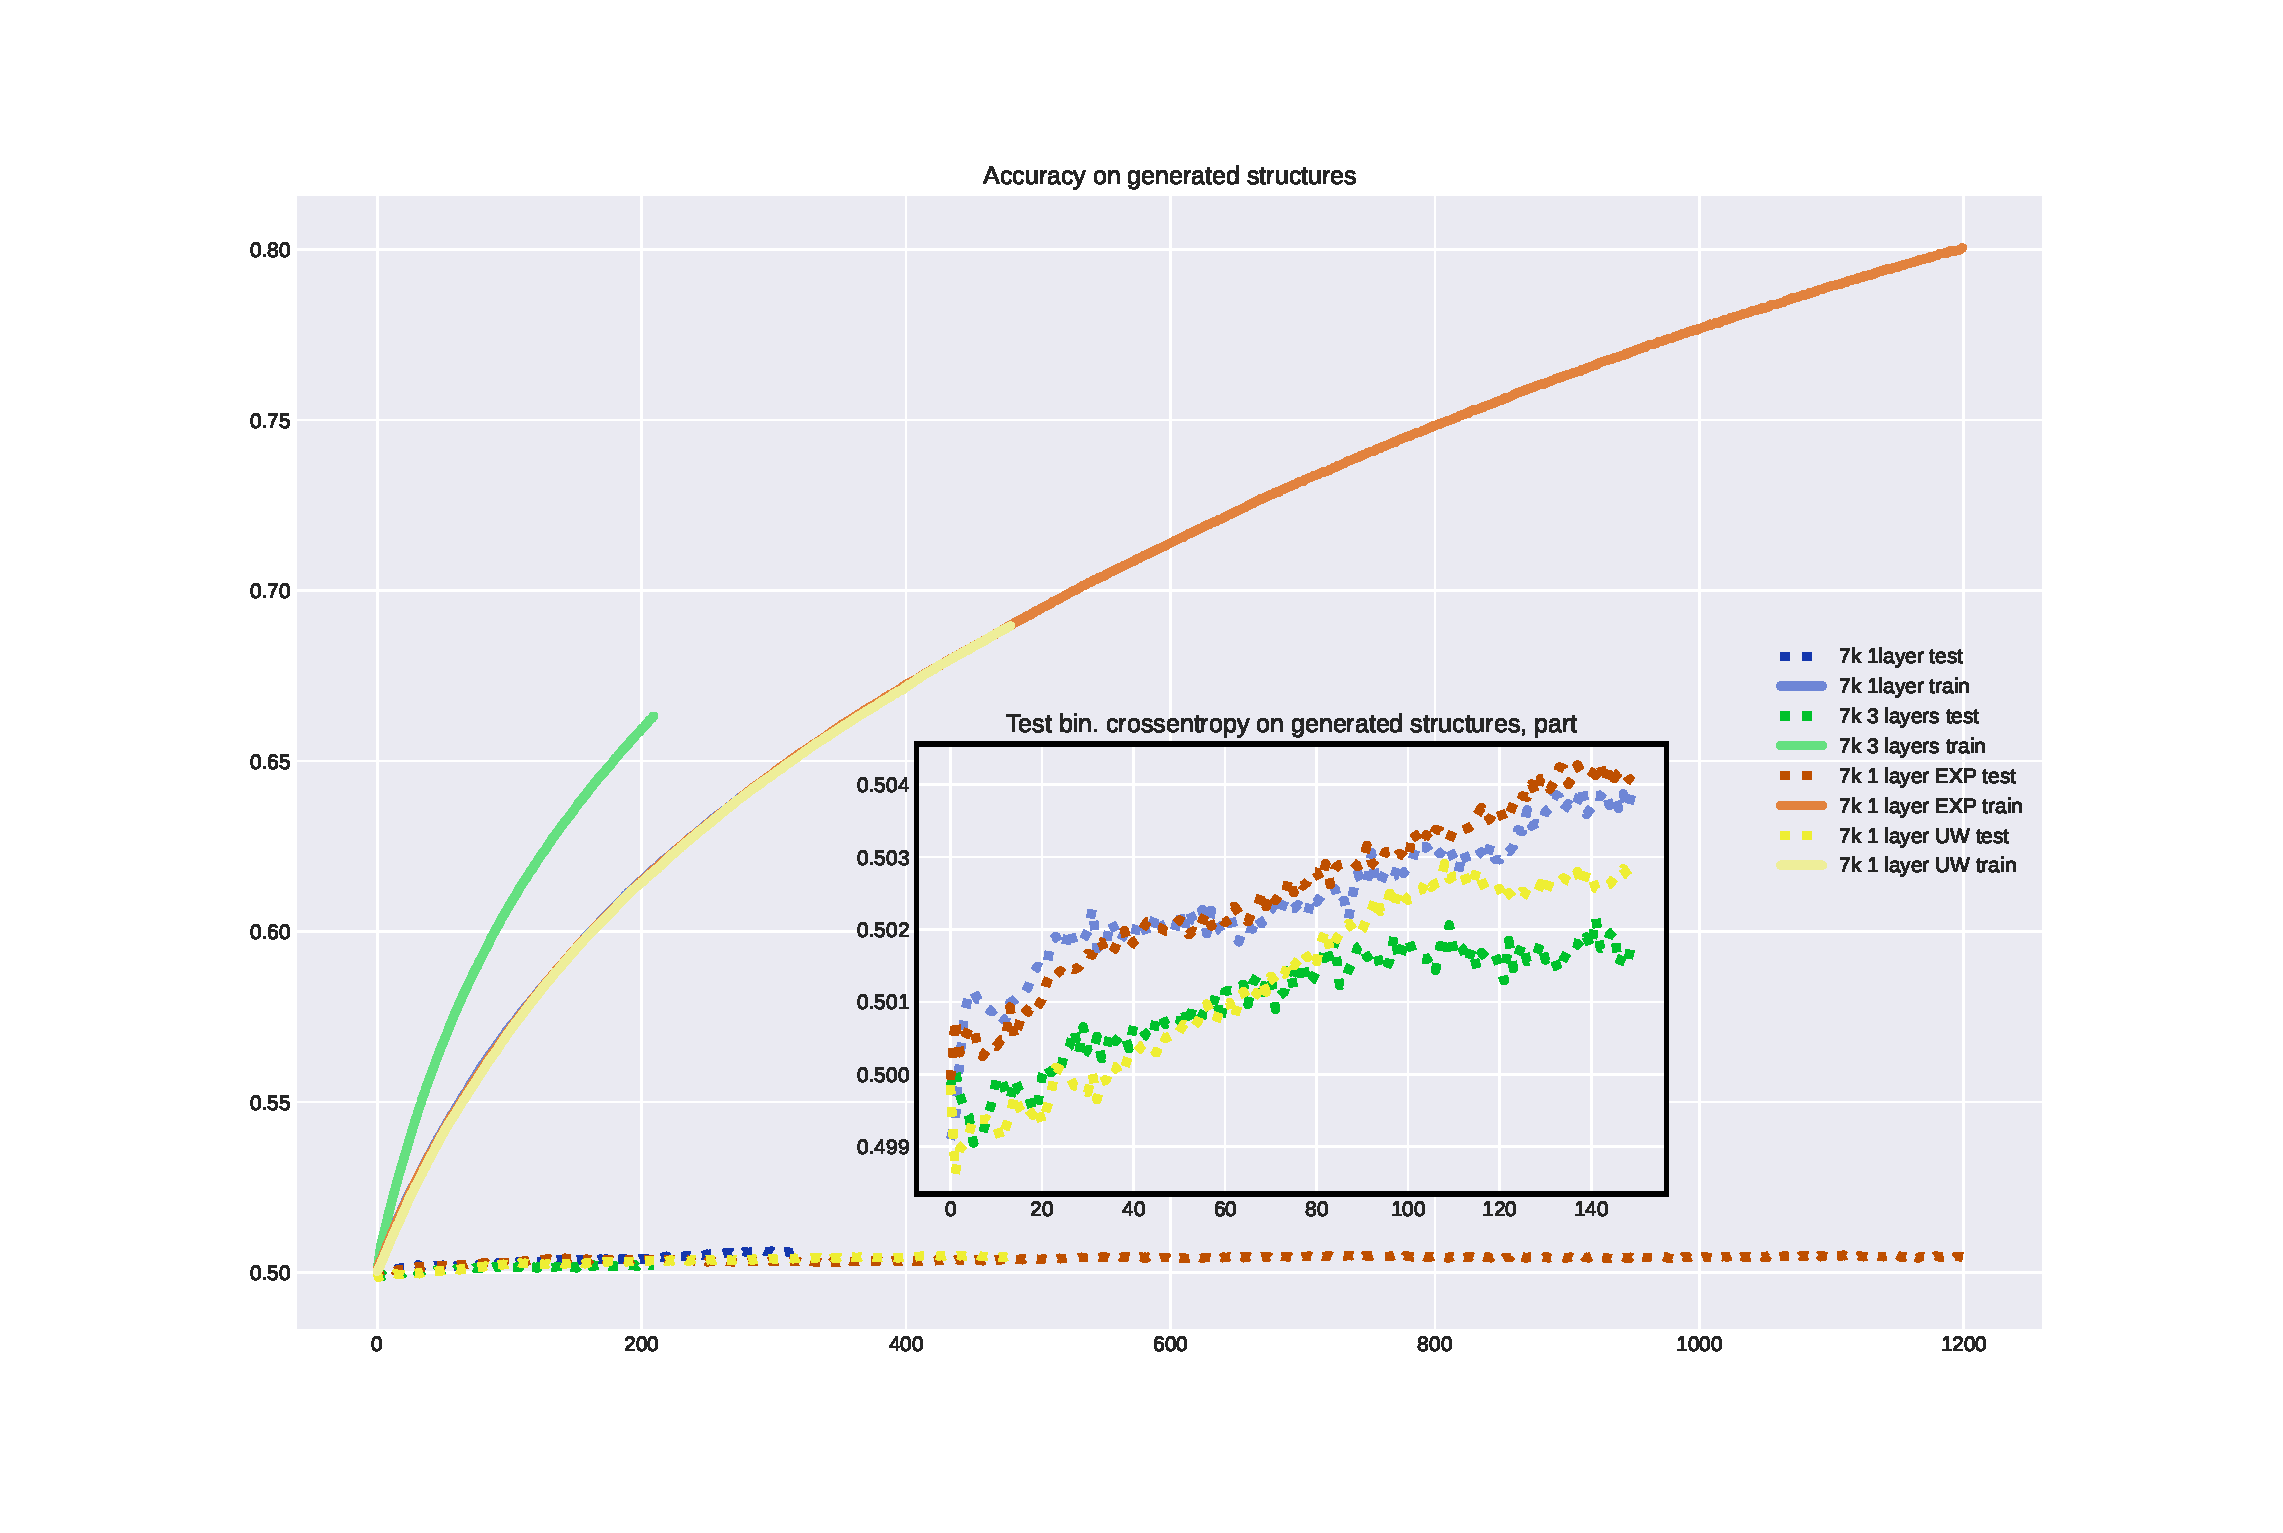
\includegraphics[scale=.500]{imgs/acc-7k.eps}
\caption{}
\label{}

\end{figure}
\begin{figure}[h!tp]
\centering
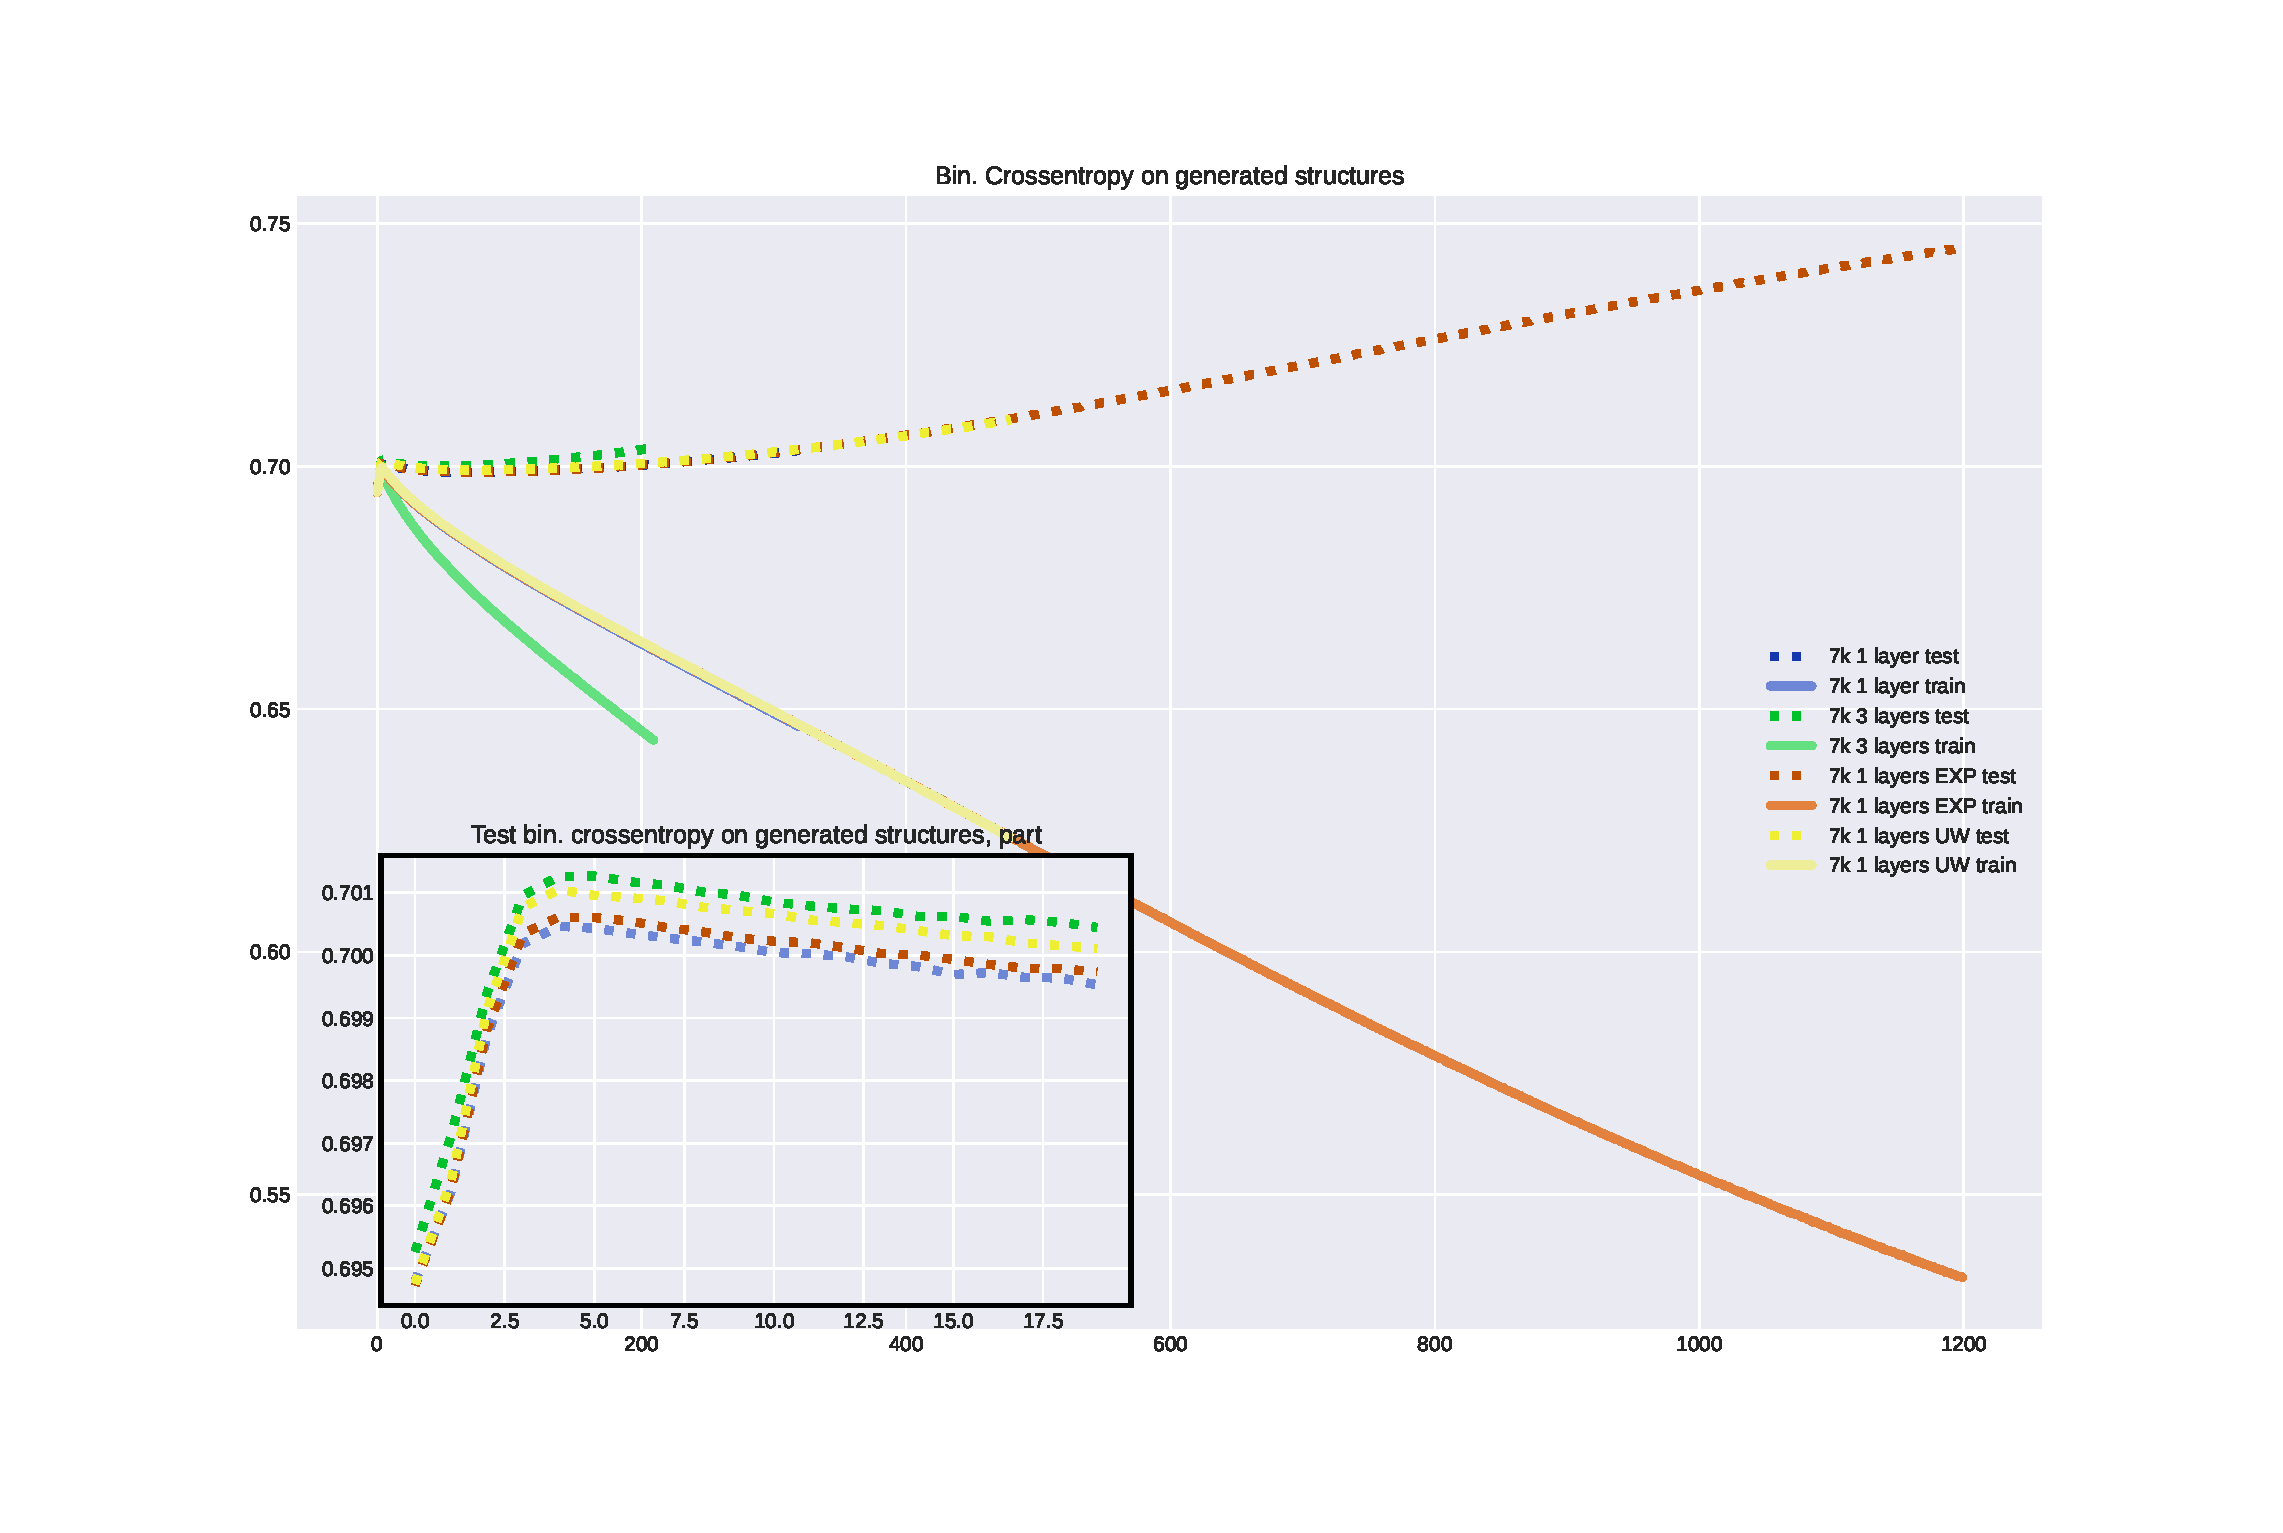
\includegraphics[scale=.500]{imgs/loss-7k.eps}
\caption{}
\label{}
\end{figure}


Обучение той же модели на 709 отражениях из 50 000 файлов дало следующие результаты: 


\begin{figure}[h!tp]
\centering
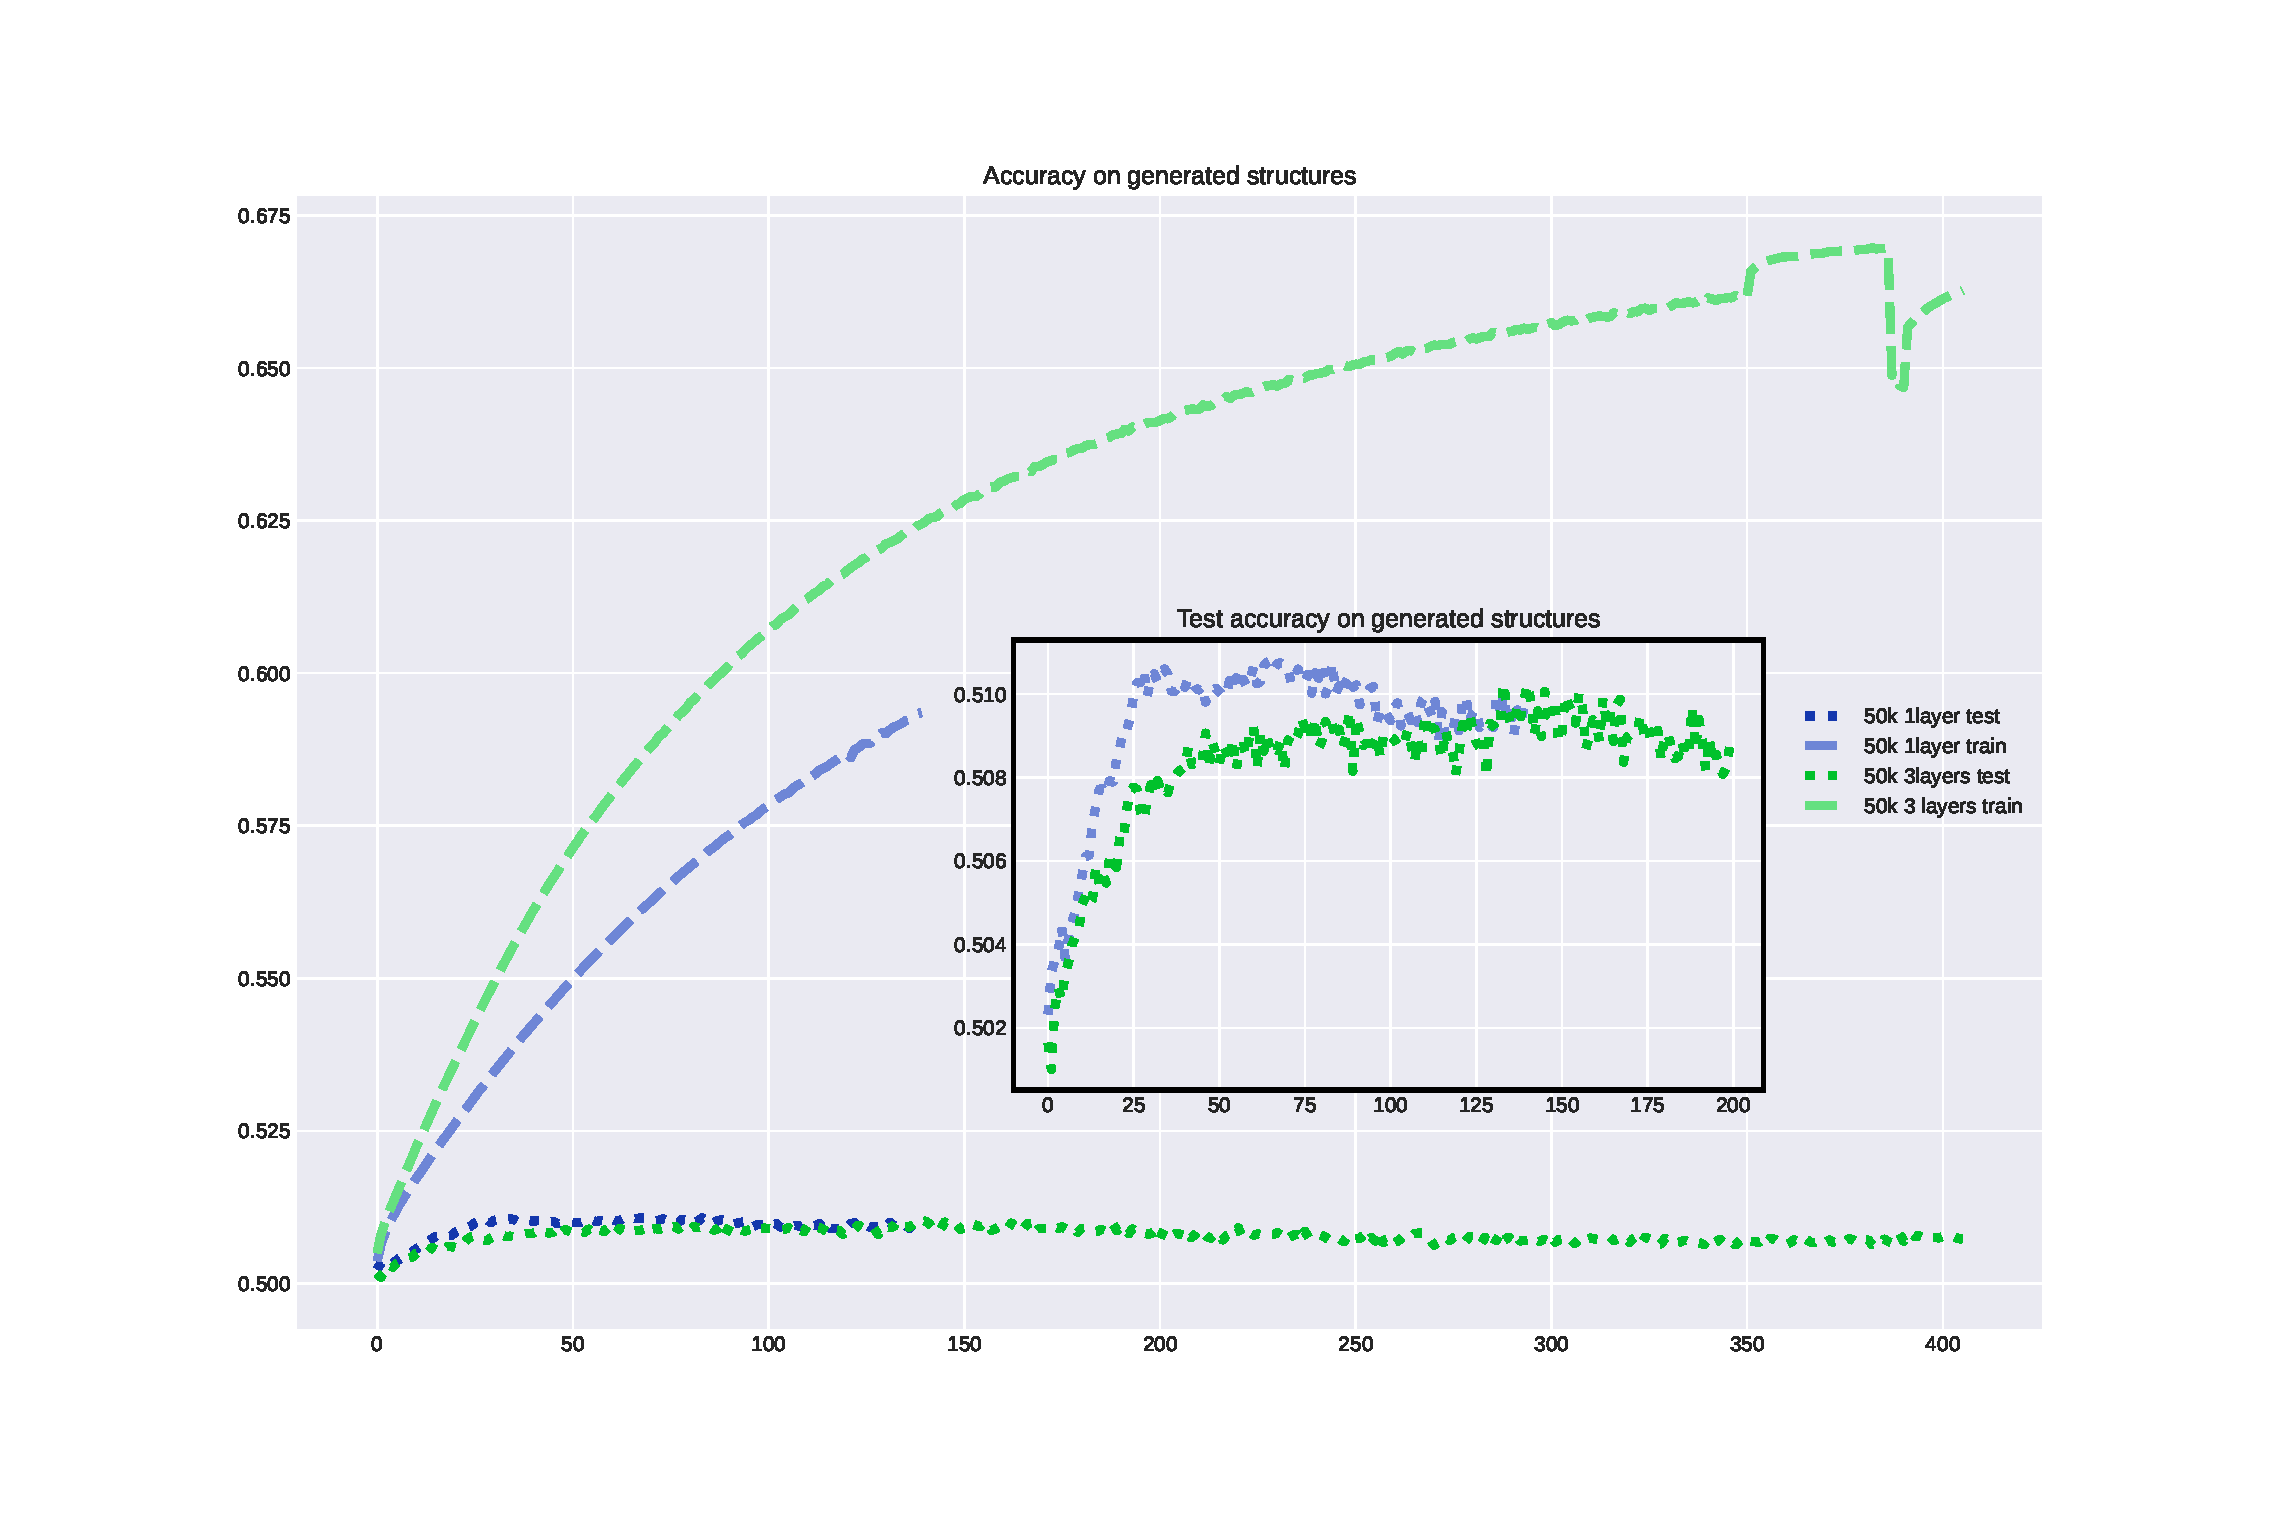
\includegraphics[scale=.500]{imgs/acc-50k.eps}
\caption{}
\label{}
\end{figure}
\begin{figure}[h!tp]
\centering
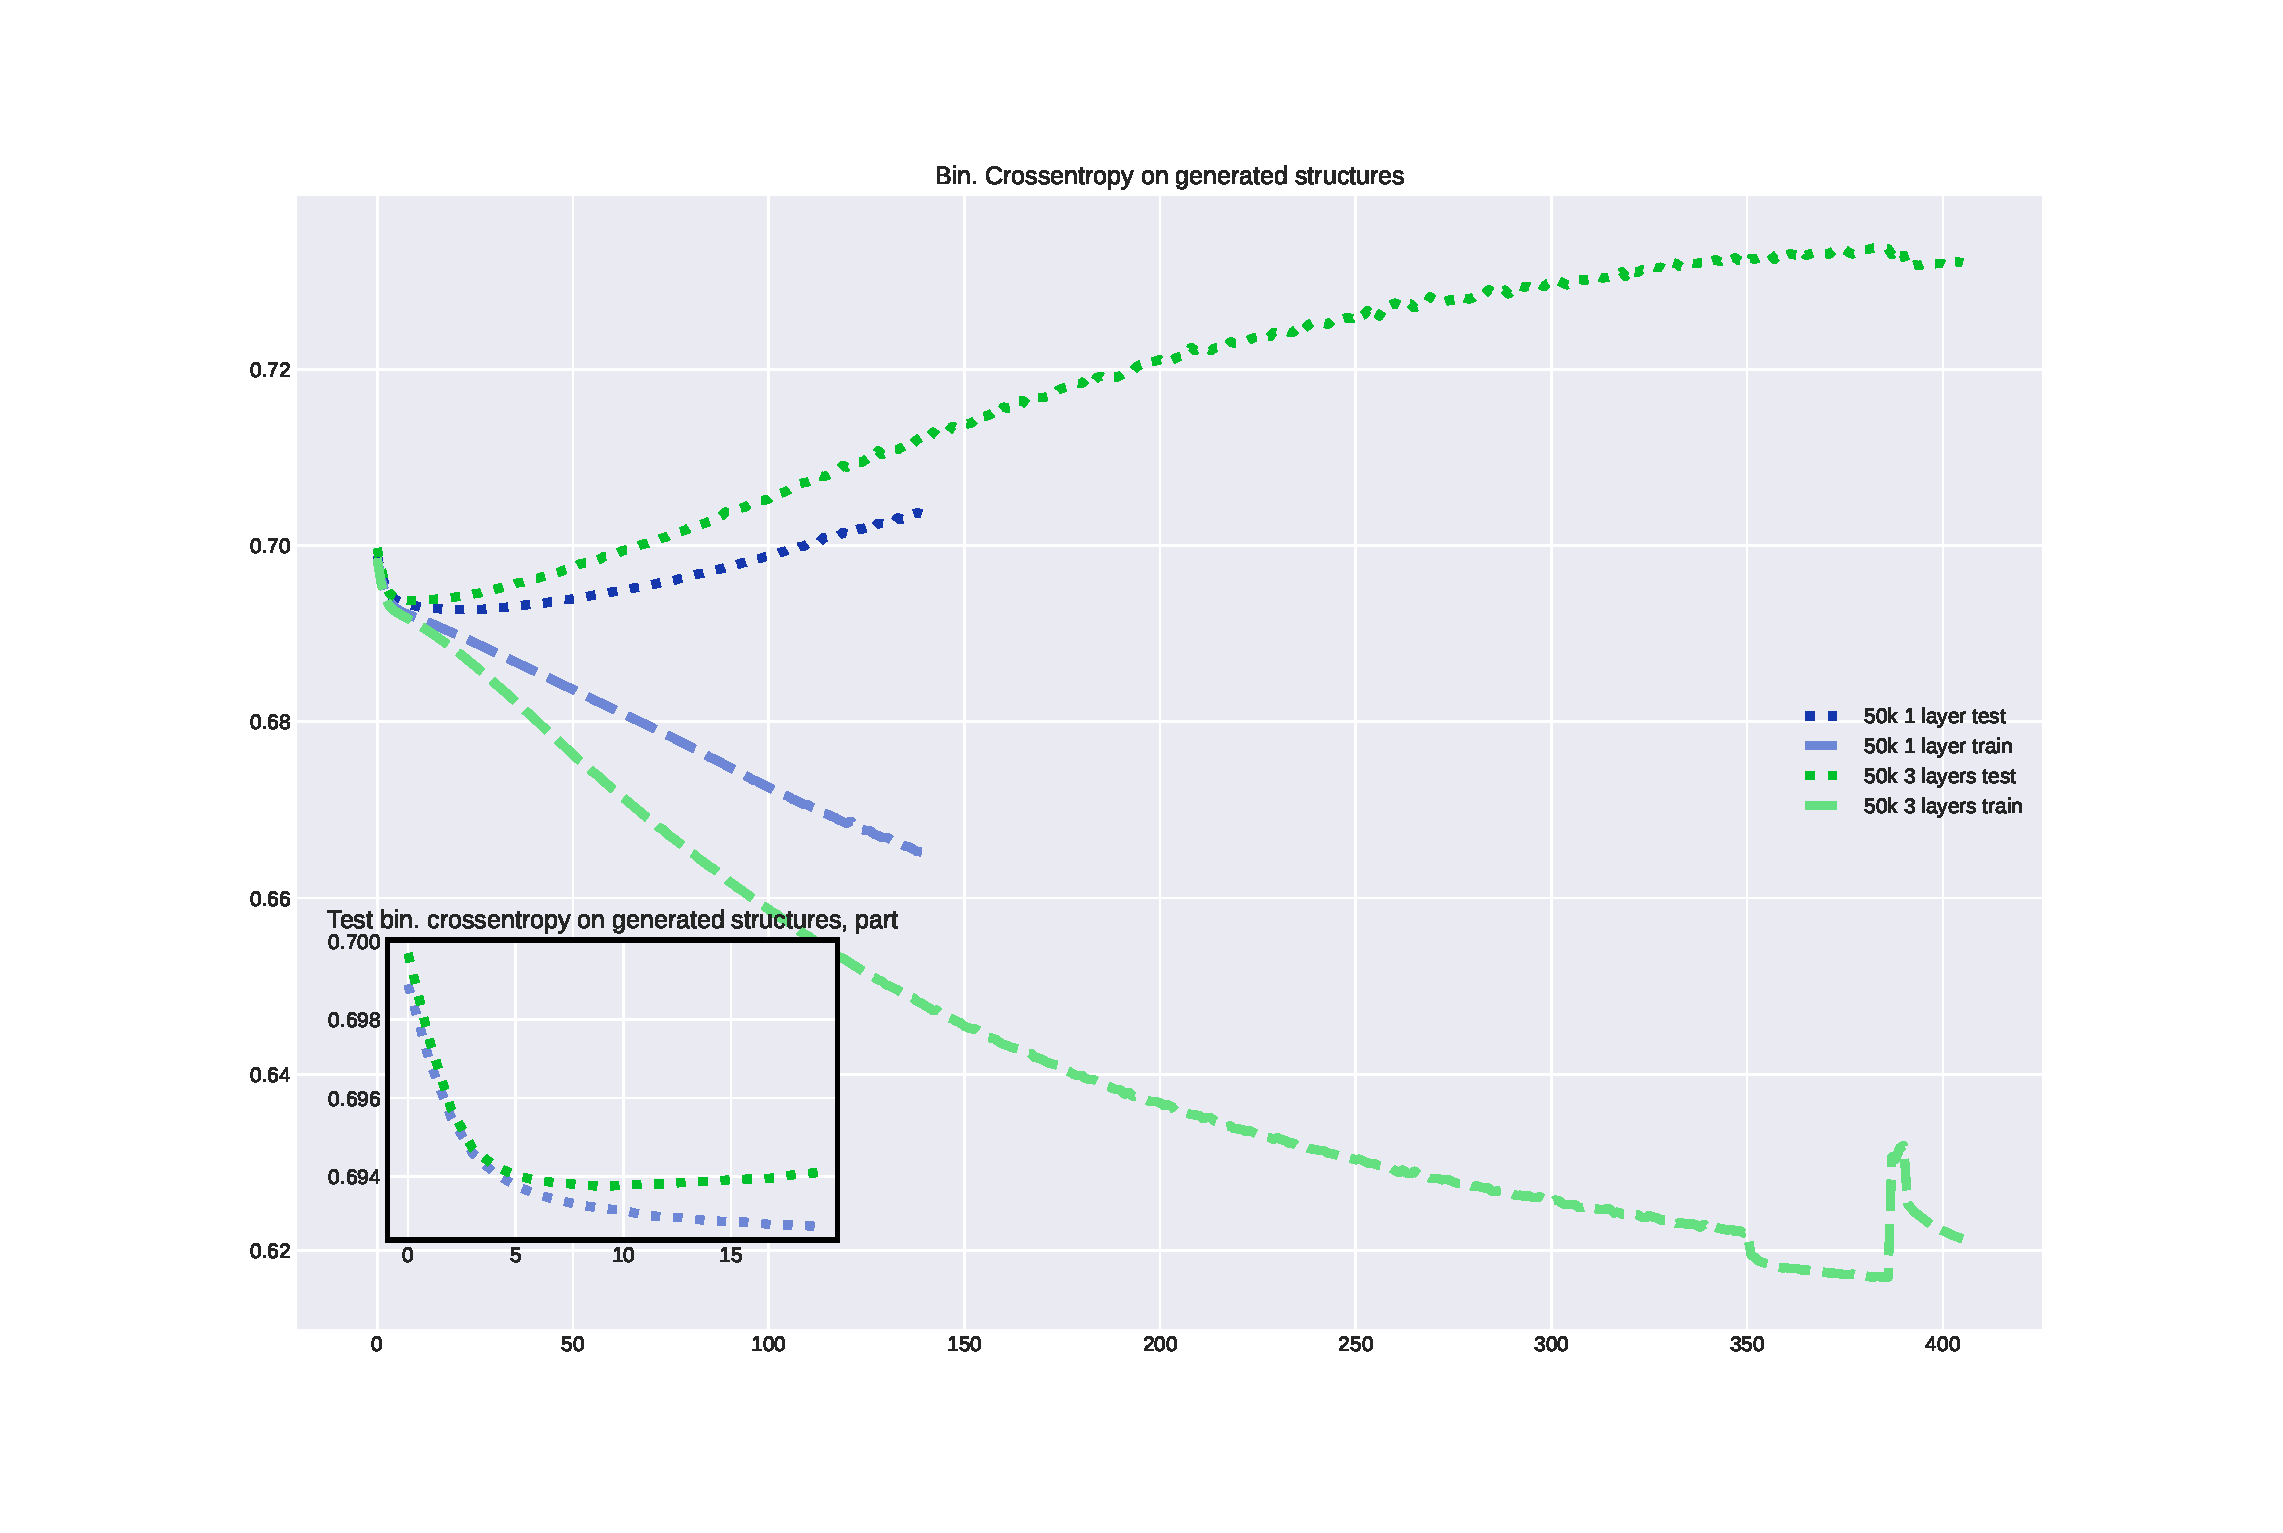
\includegraphics[scale=.500]{imgs/loss-50k.eps}
\caption{}
\label{}
\end{figure}

Зависимость качества обучения от размера датасета
\begin{figure}[h!tp]
\centering
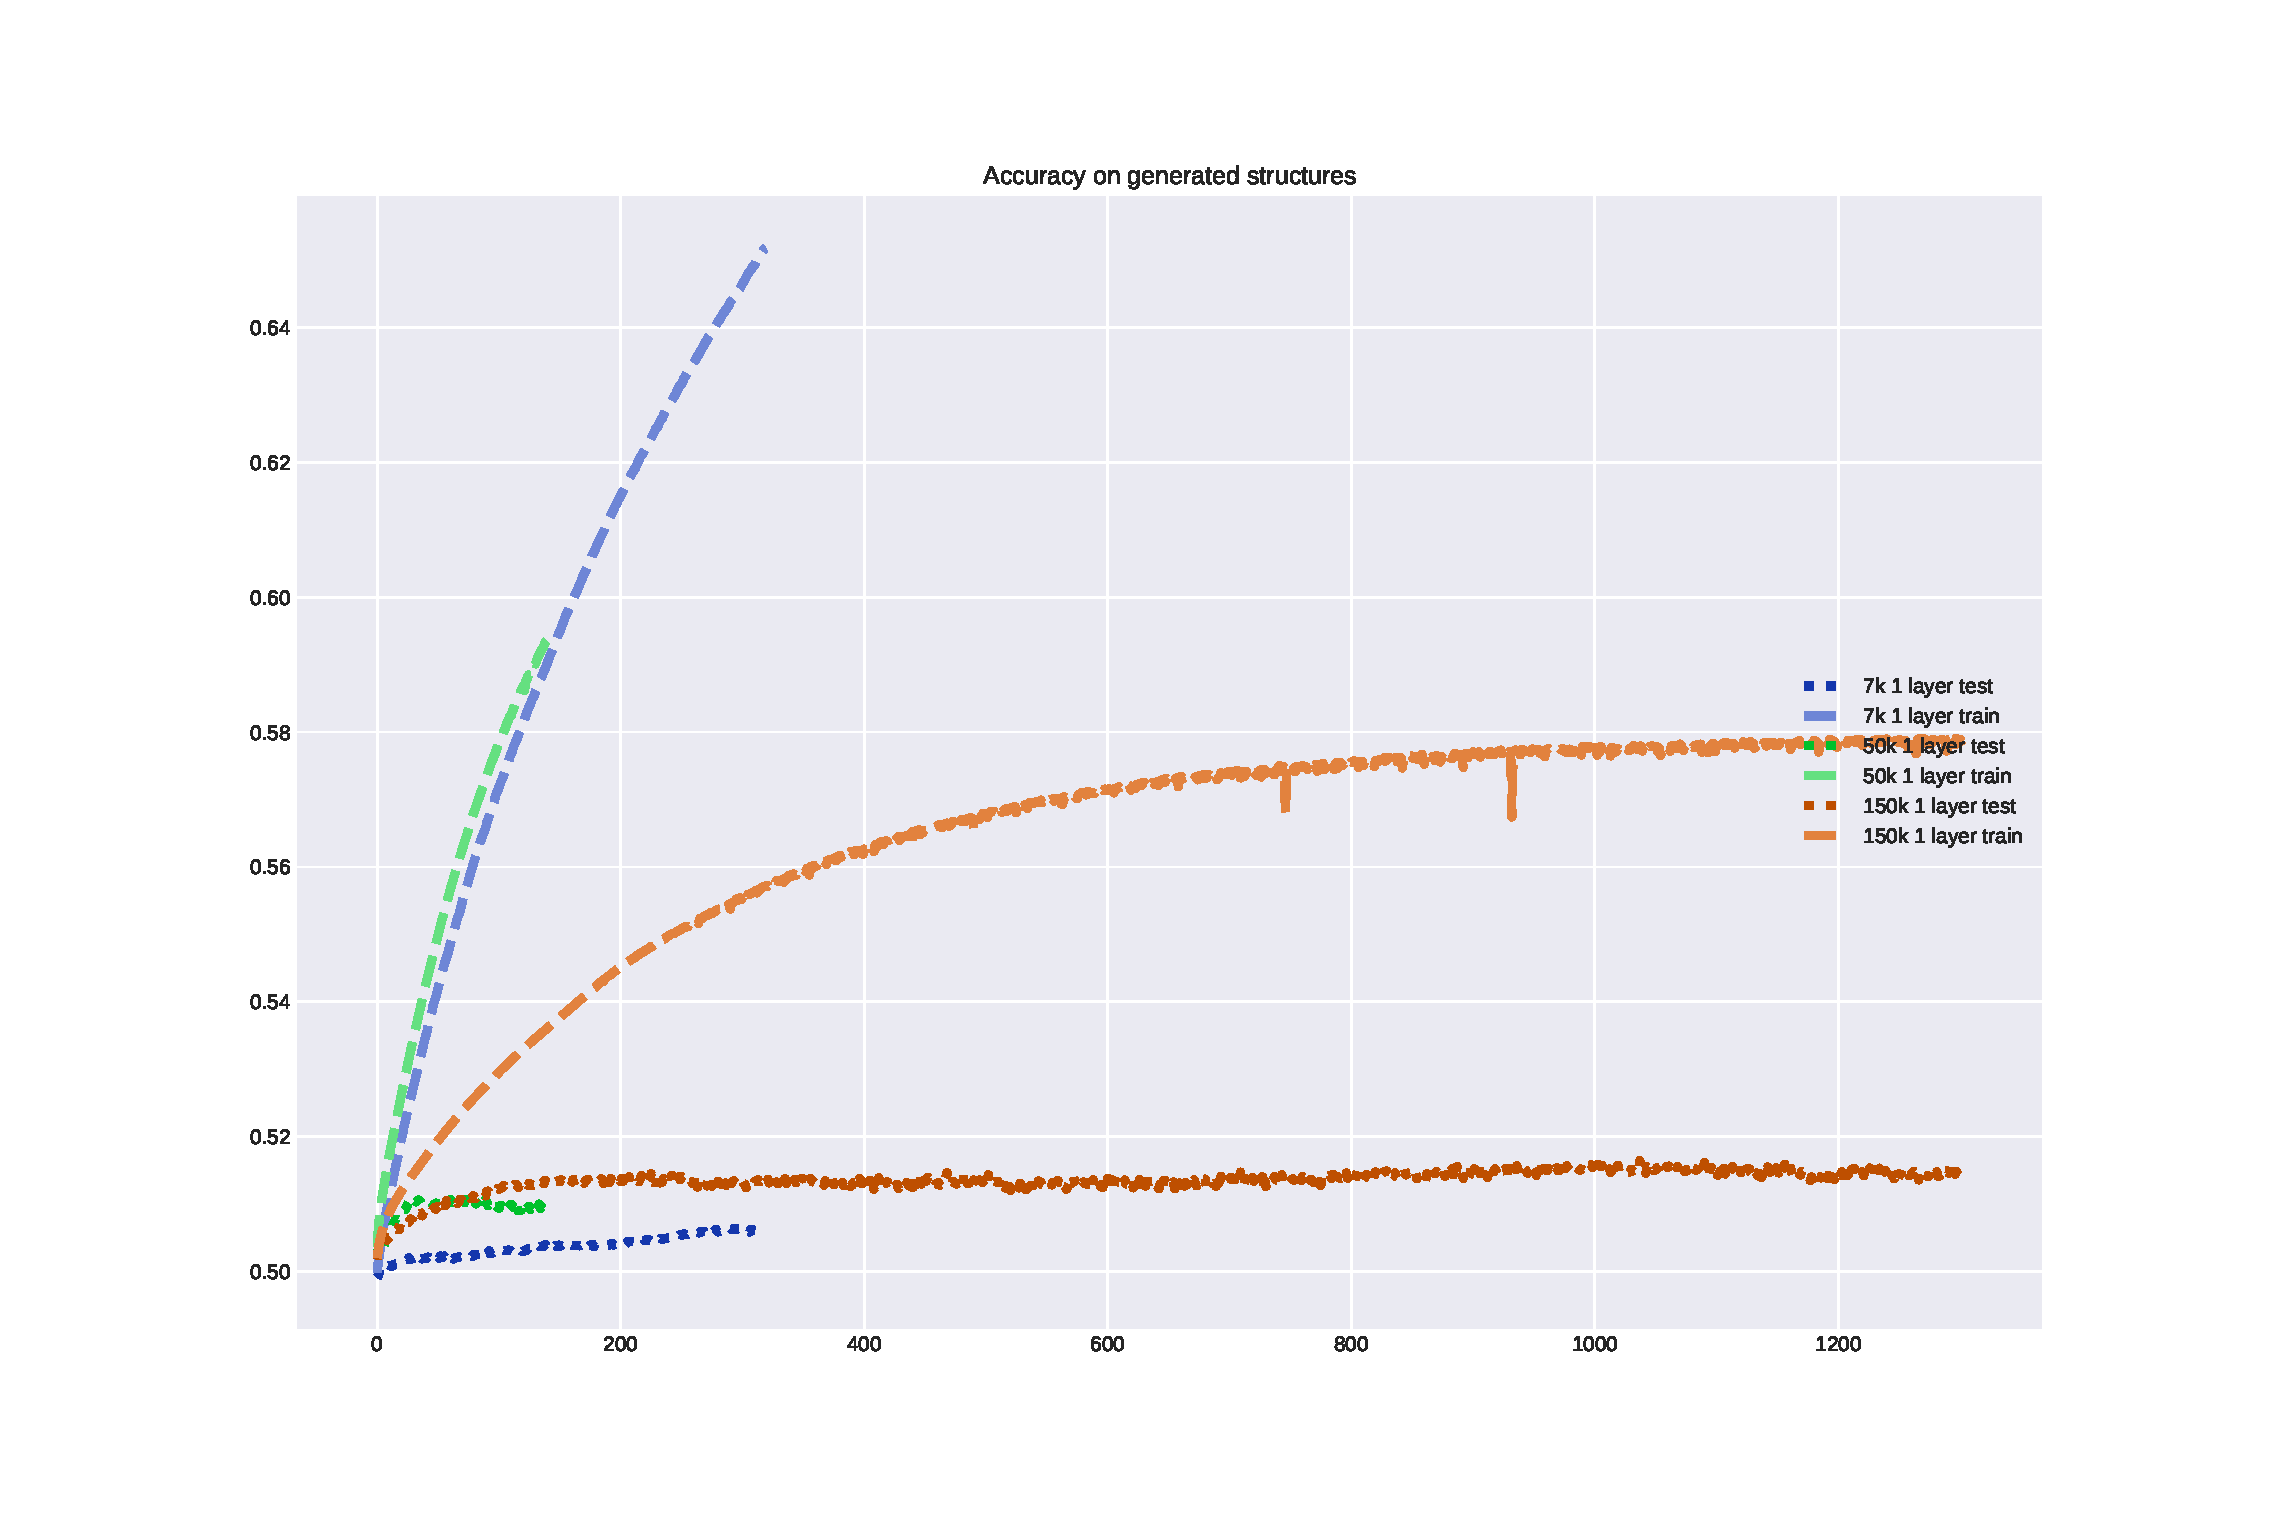
\includegraphics[scale=.500]{imgs/acc-1l_ndata.eps}
\caption{}
\label{}
\end{figure}

\begin{figure}[h!tp]
\centering
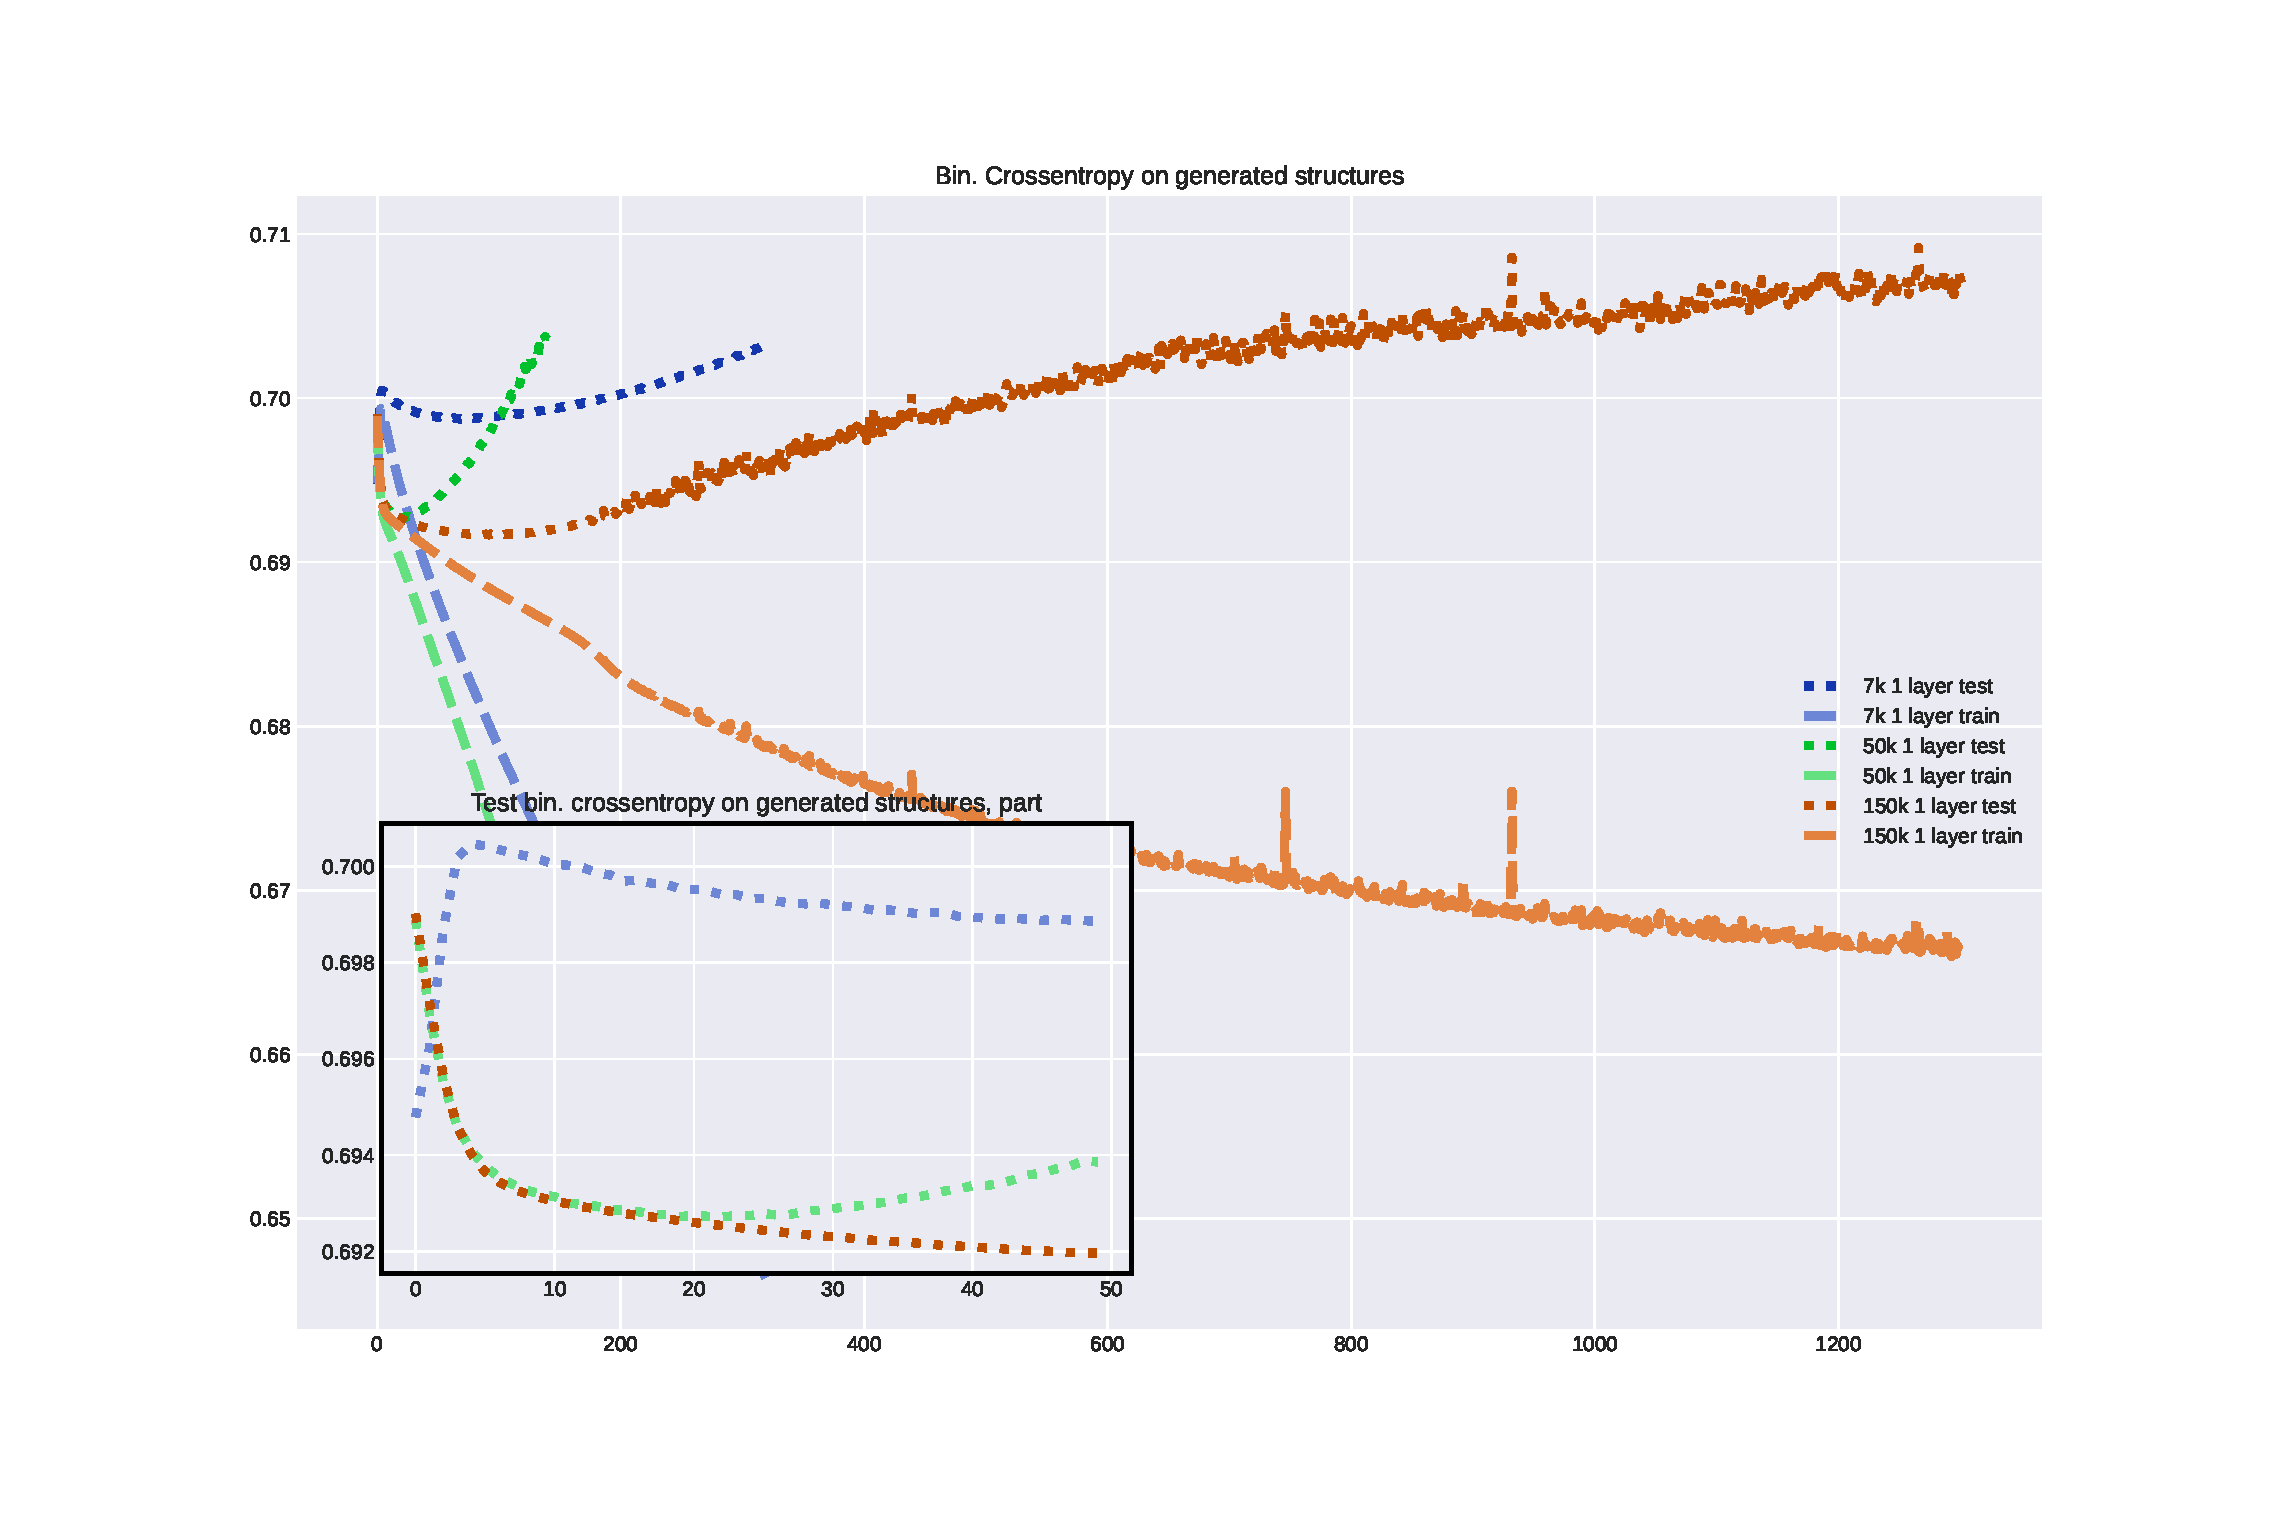
\includegraphics[scale=.500]{imgs/loss-1l_ndata.eps}
\caption{}
\label{}
\end{figure}

То же для 3 слоев
\begin{figure}[h!tp]
\centering
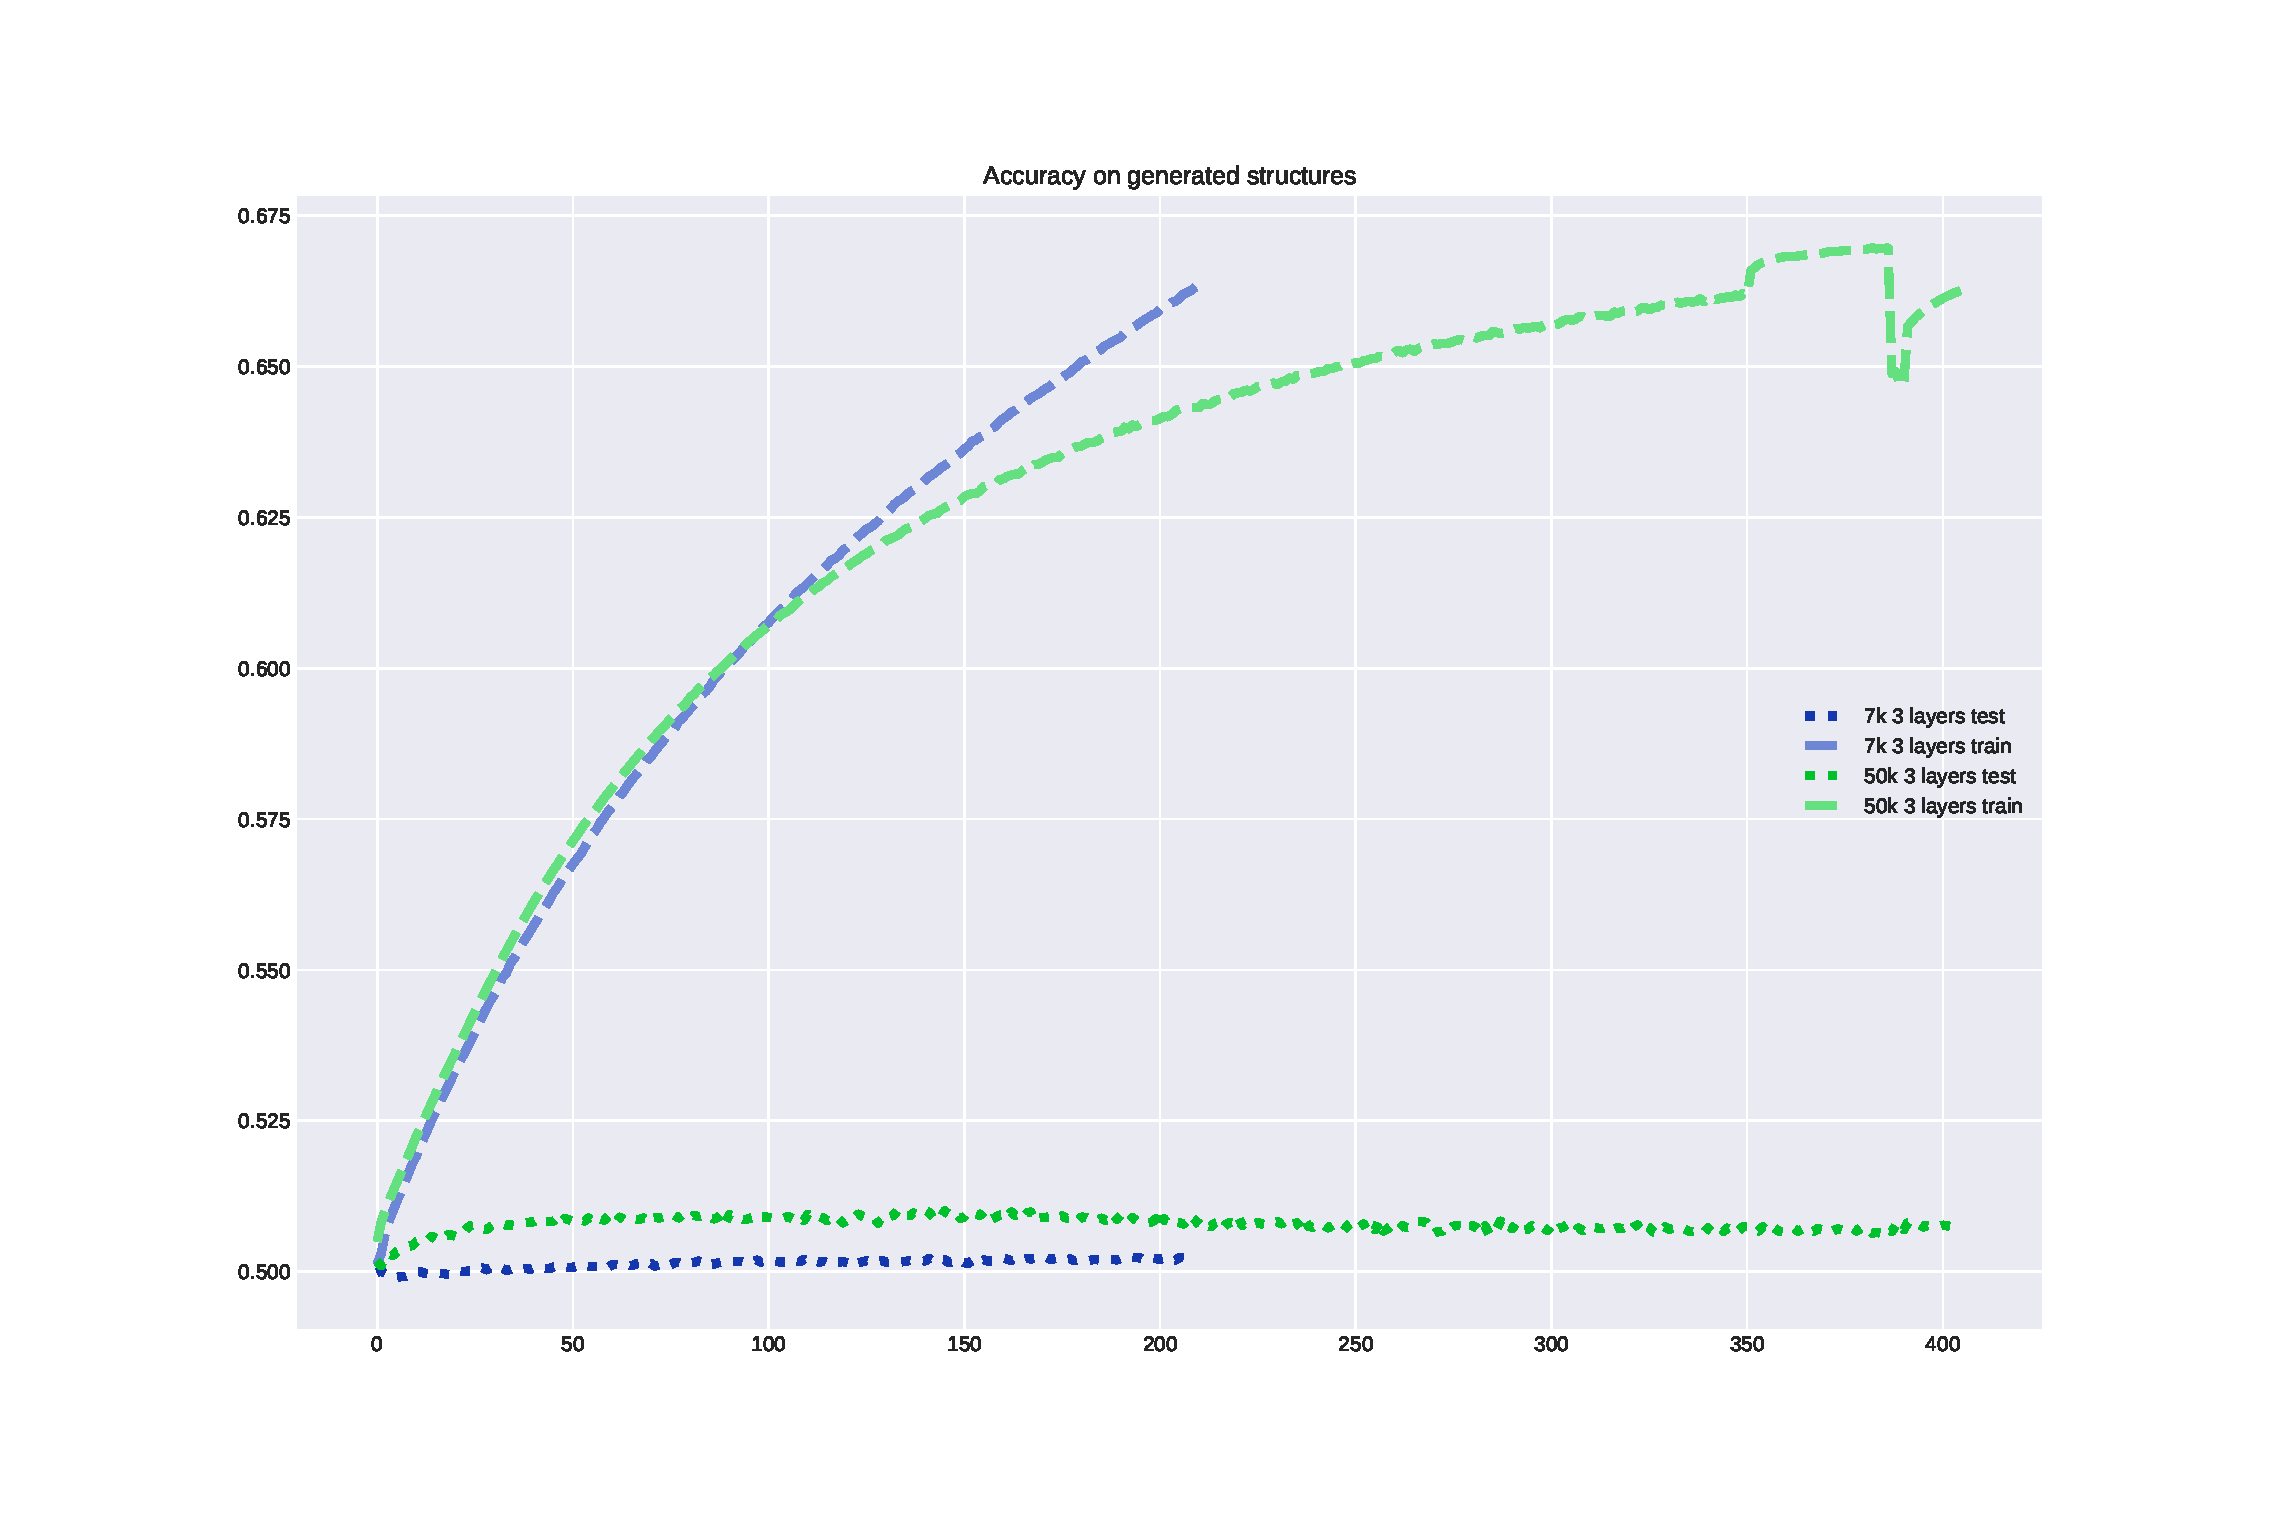
\includegraphics[scale=.500]{imgs/acc-3l_ndata.eps}
\caption{}
\label{}
\end{figure}


\begin{figure}[h!tp]
\centering
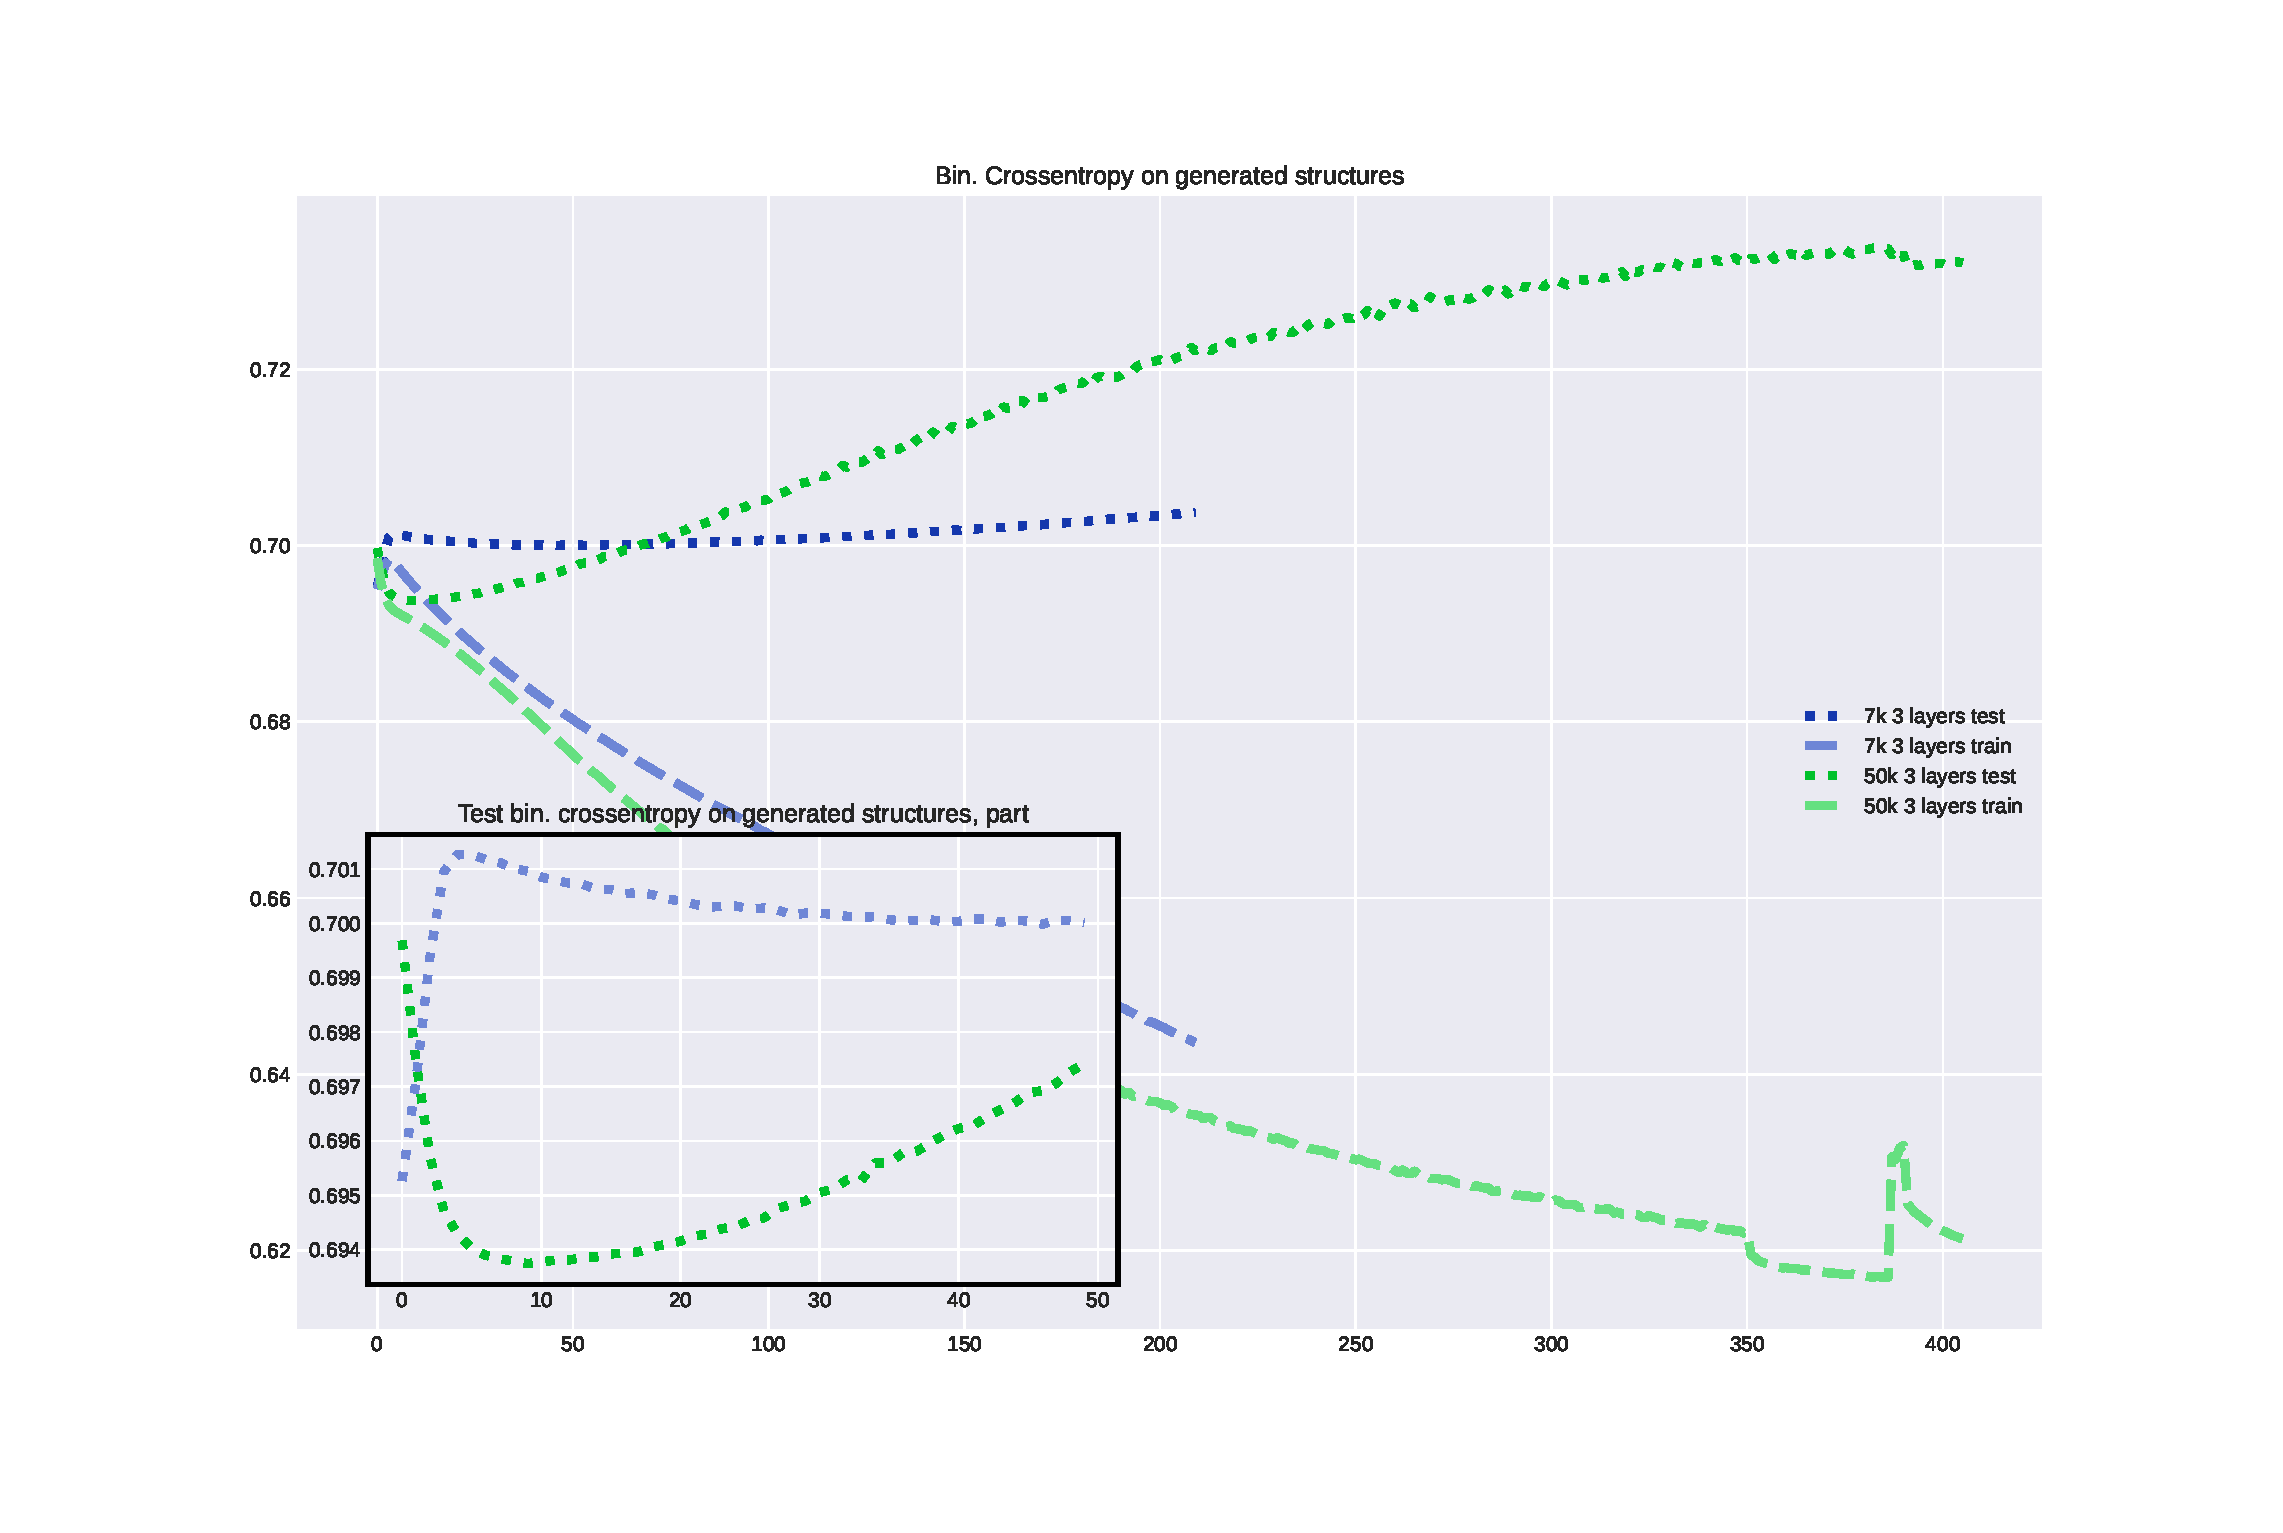
\includegraphics[scale=.500]{imgs/loss-3l_ndata.eps}
\caption{}
\label{}
\end{figure}

Зависимость качества обучения от типа весов
\begin{figure}[h!tp]
\centering
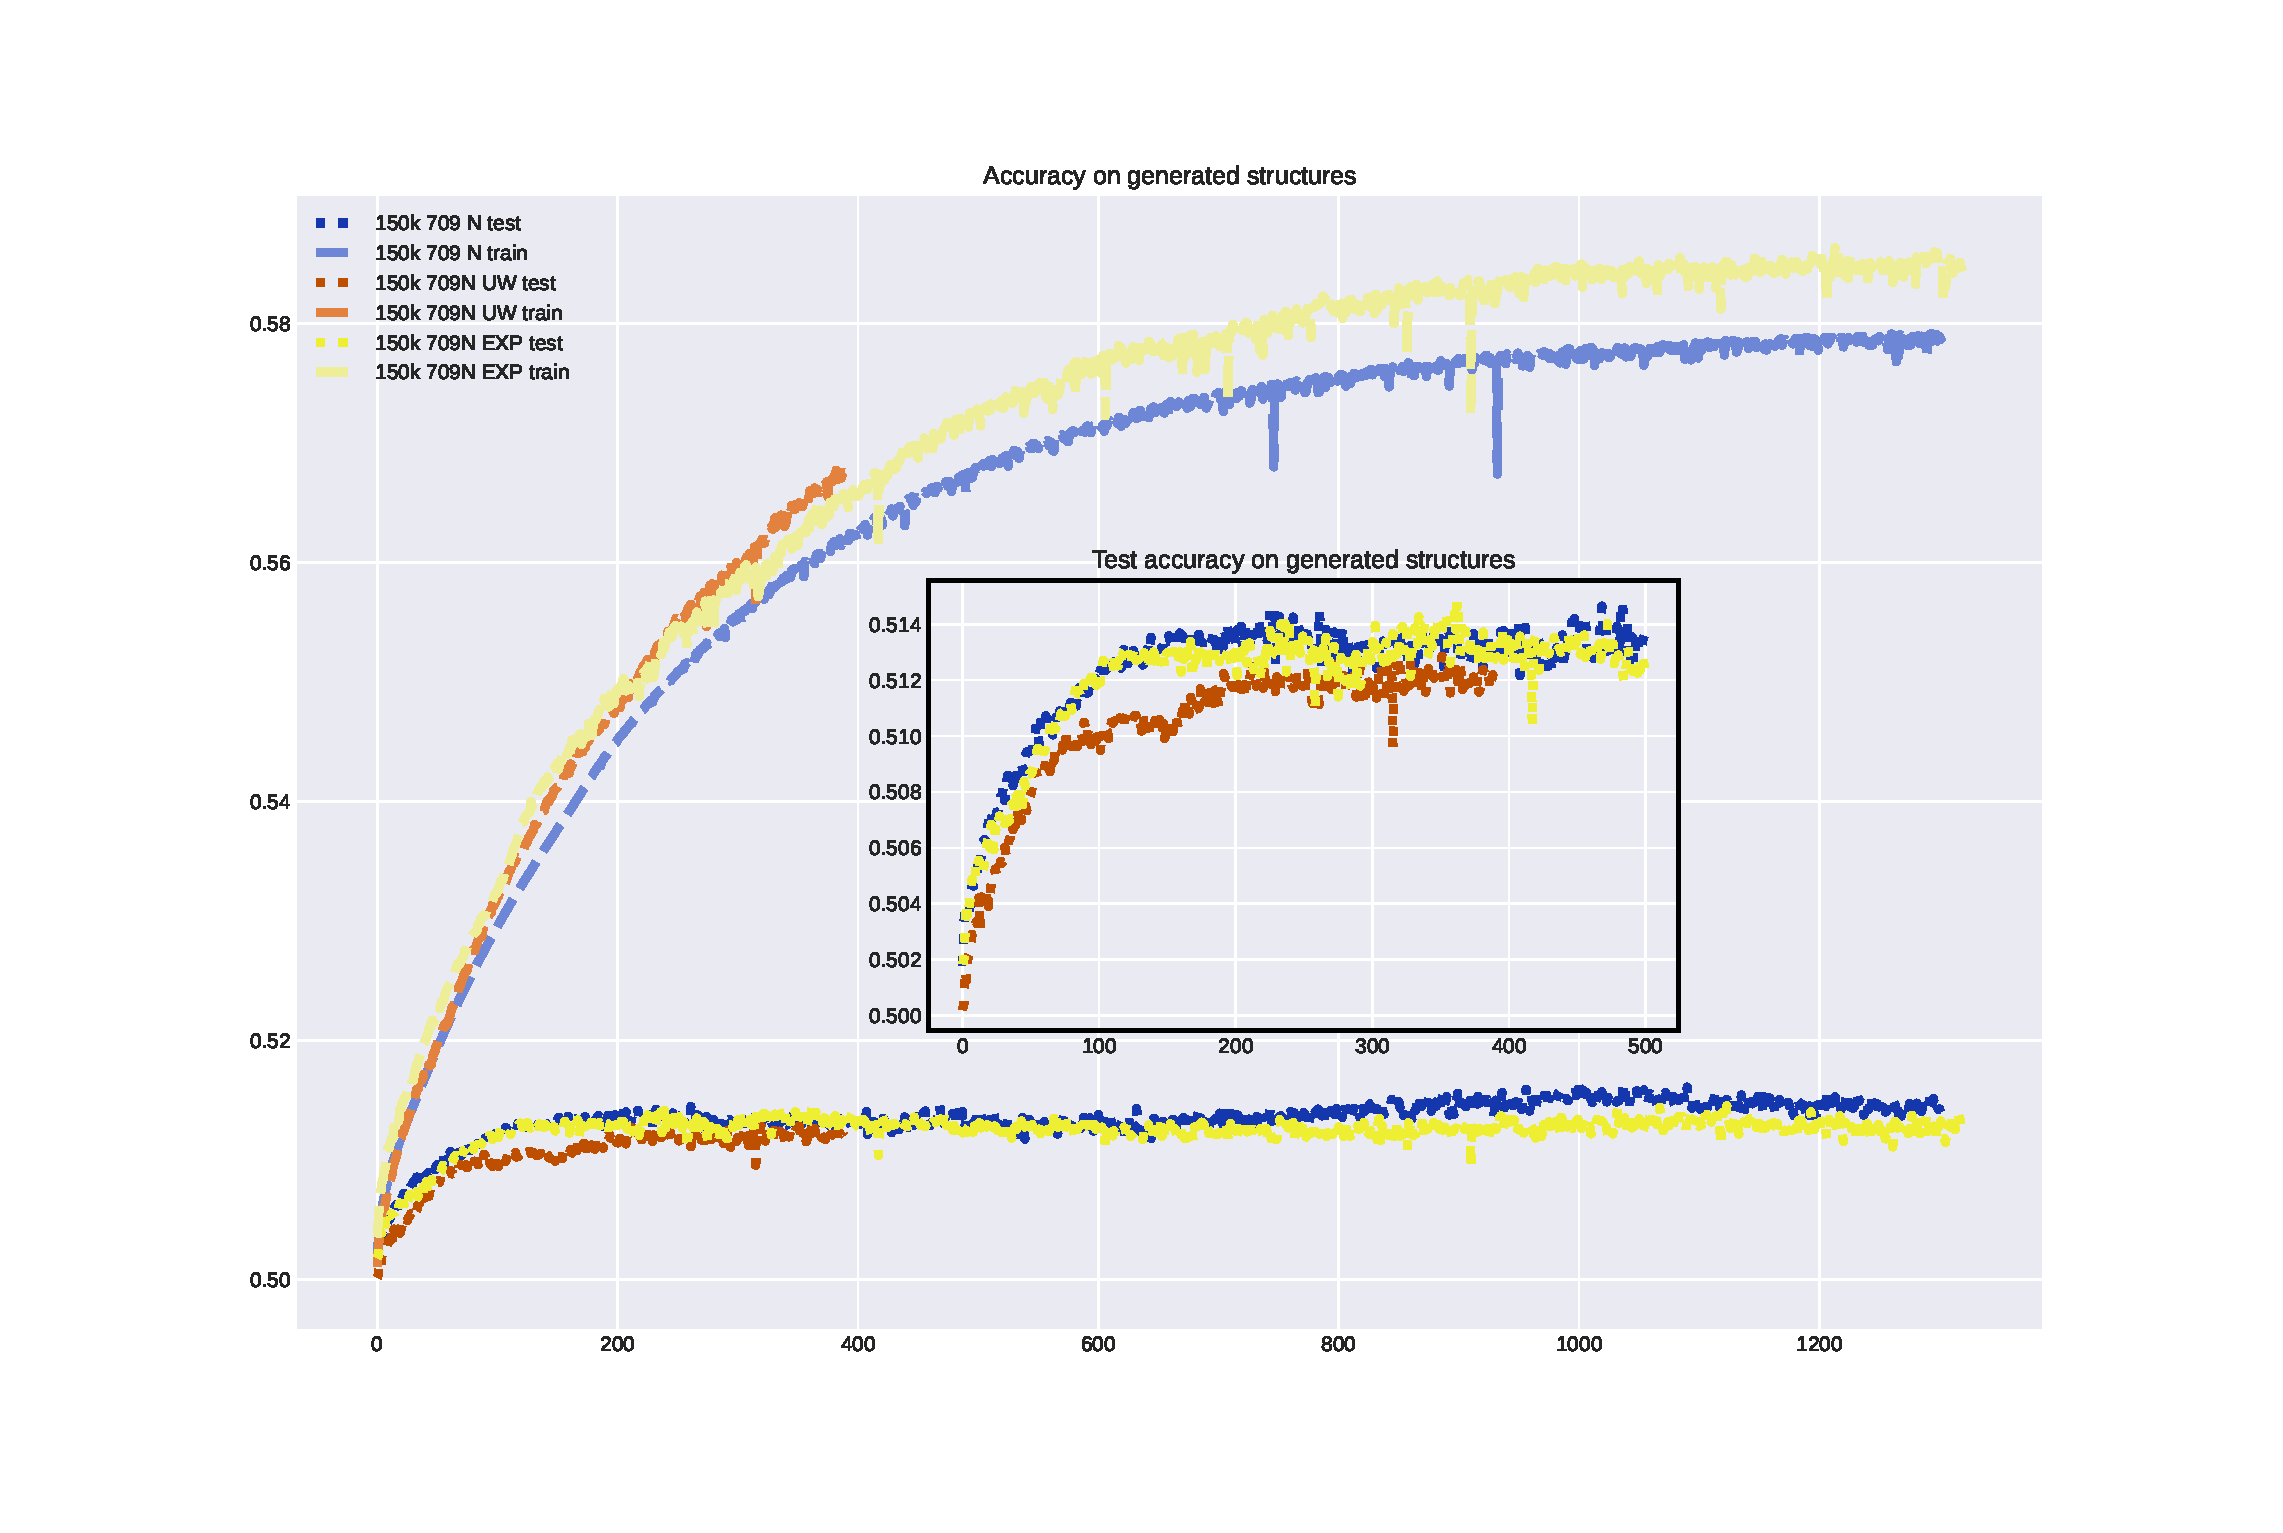
\includegraphics[scale=.500]{imgs/acc-weight.eps}
\caption{}
\label{}
\end{figure}

\begin{figure}[h!tp]
\centering
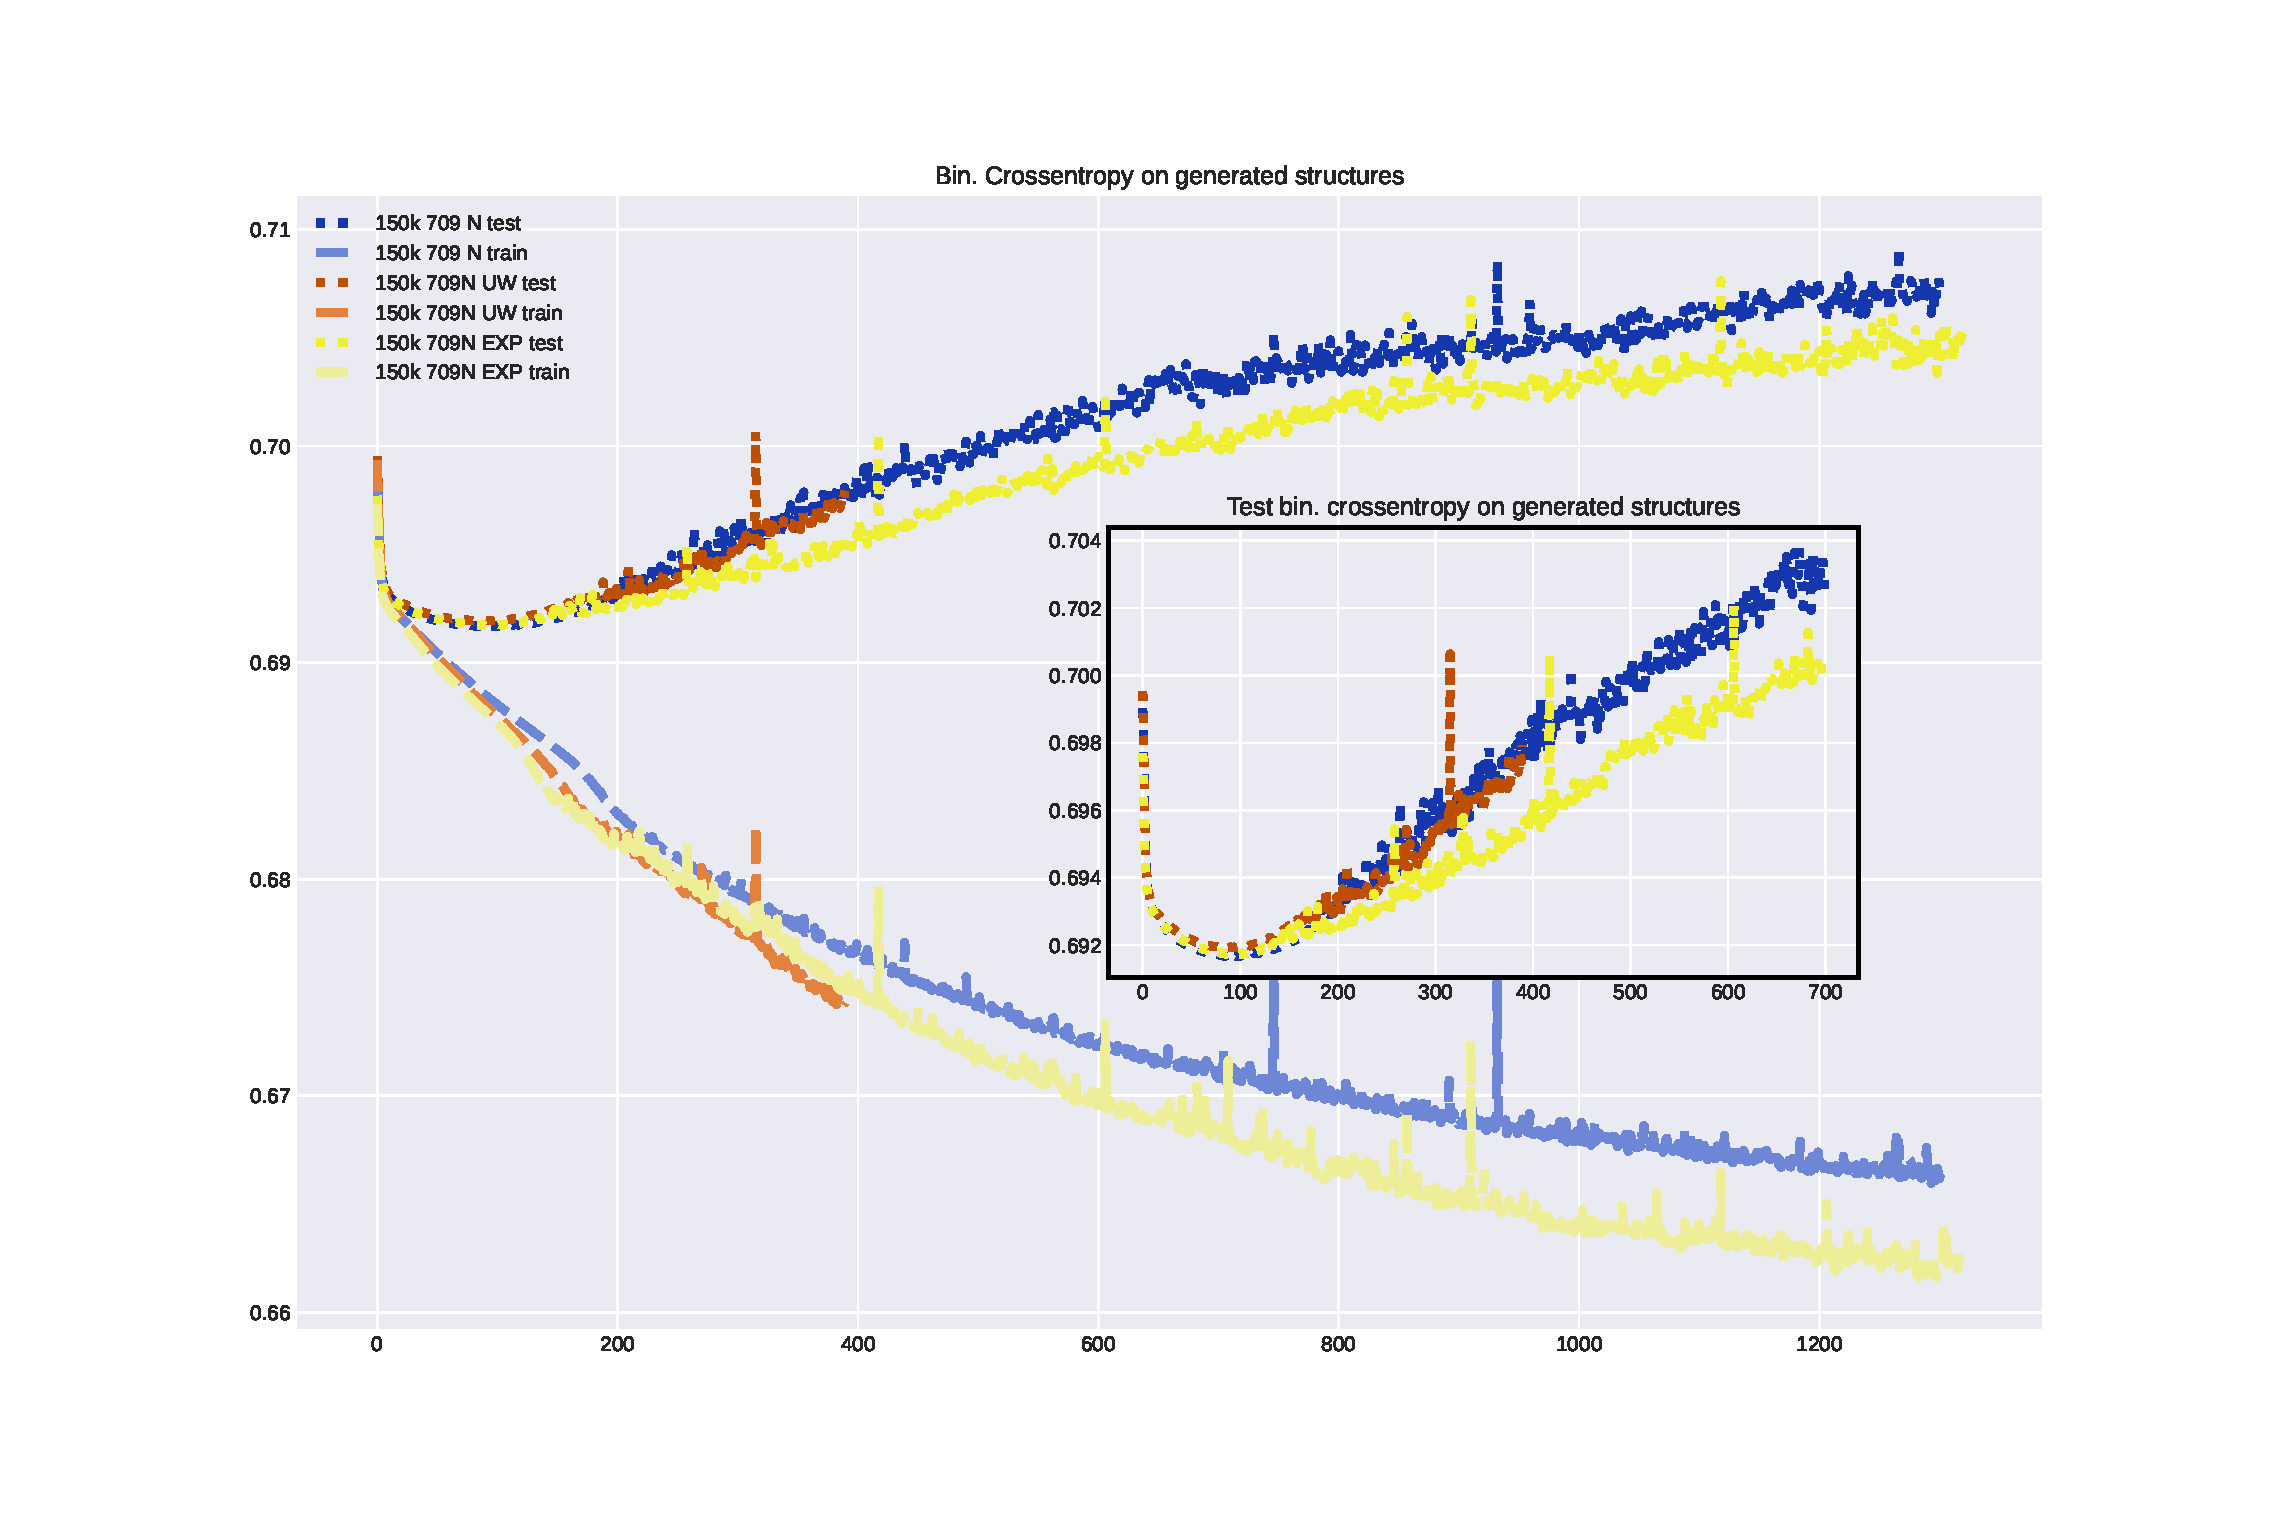
\includegraphics[scale=.500]{imgs/loss-weight.eps}
\caption{}
\label{}
\end{figure}


\begin{figure}[h!tp]
\centering
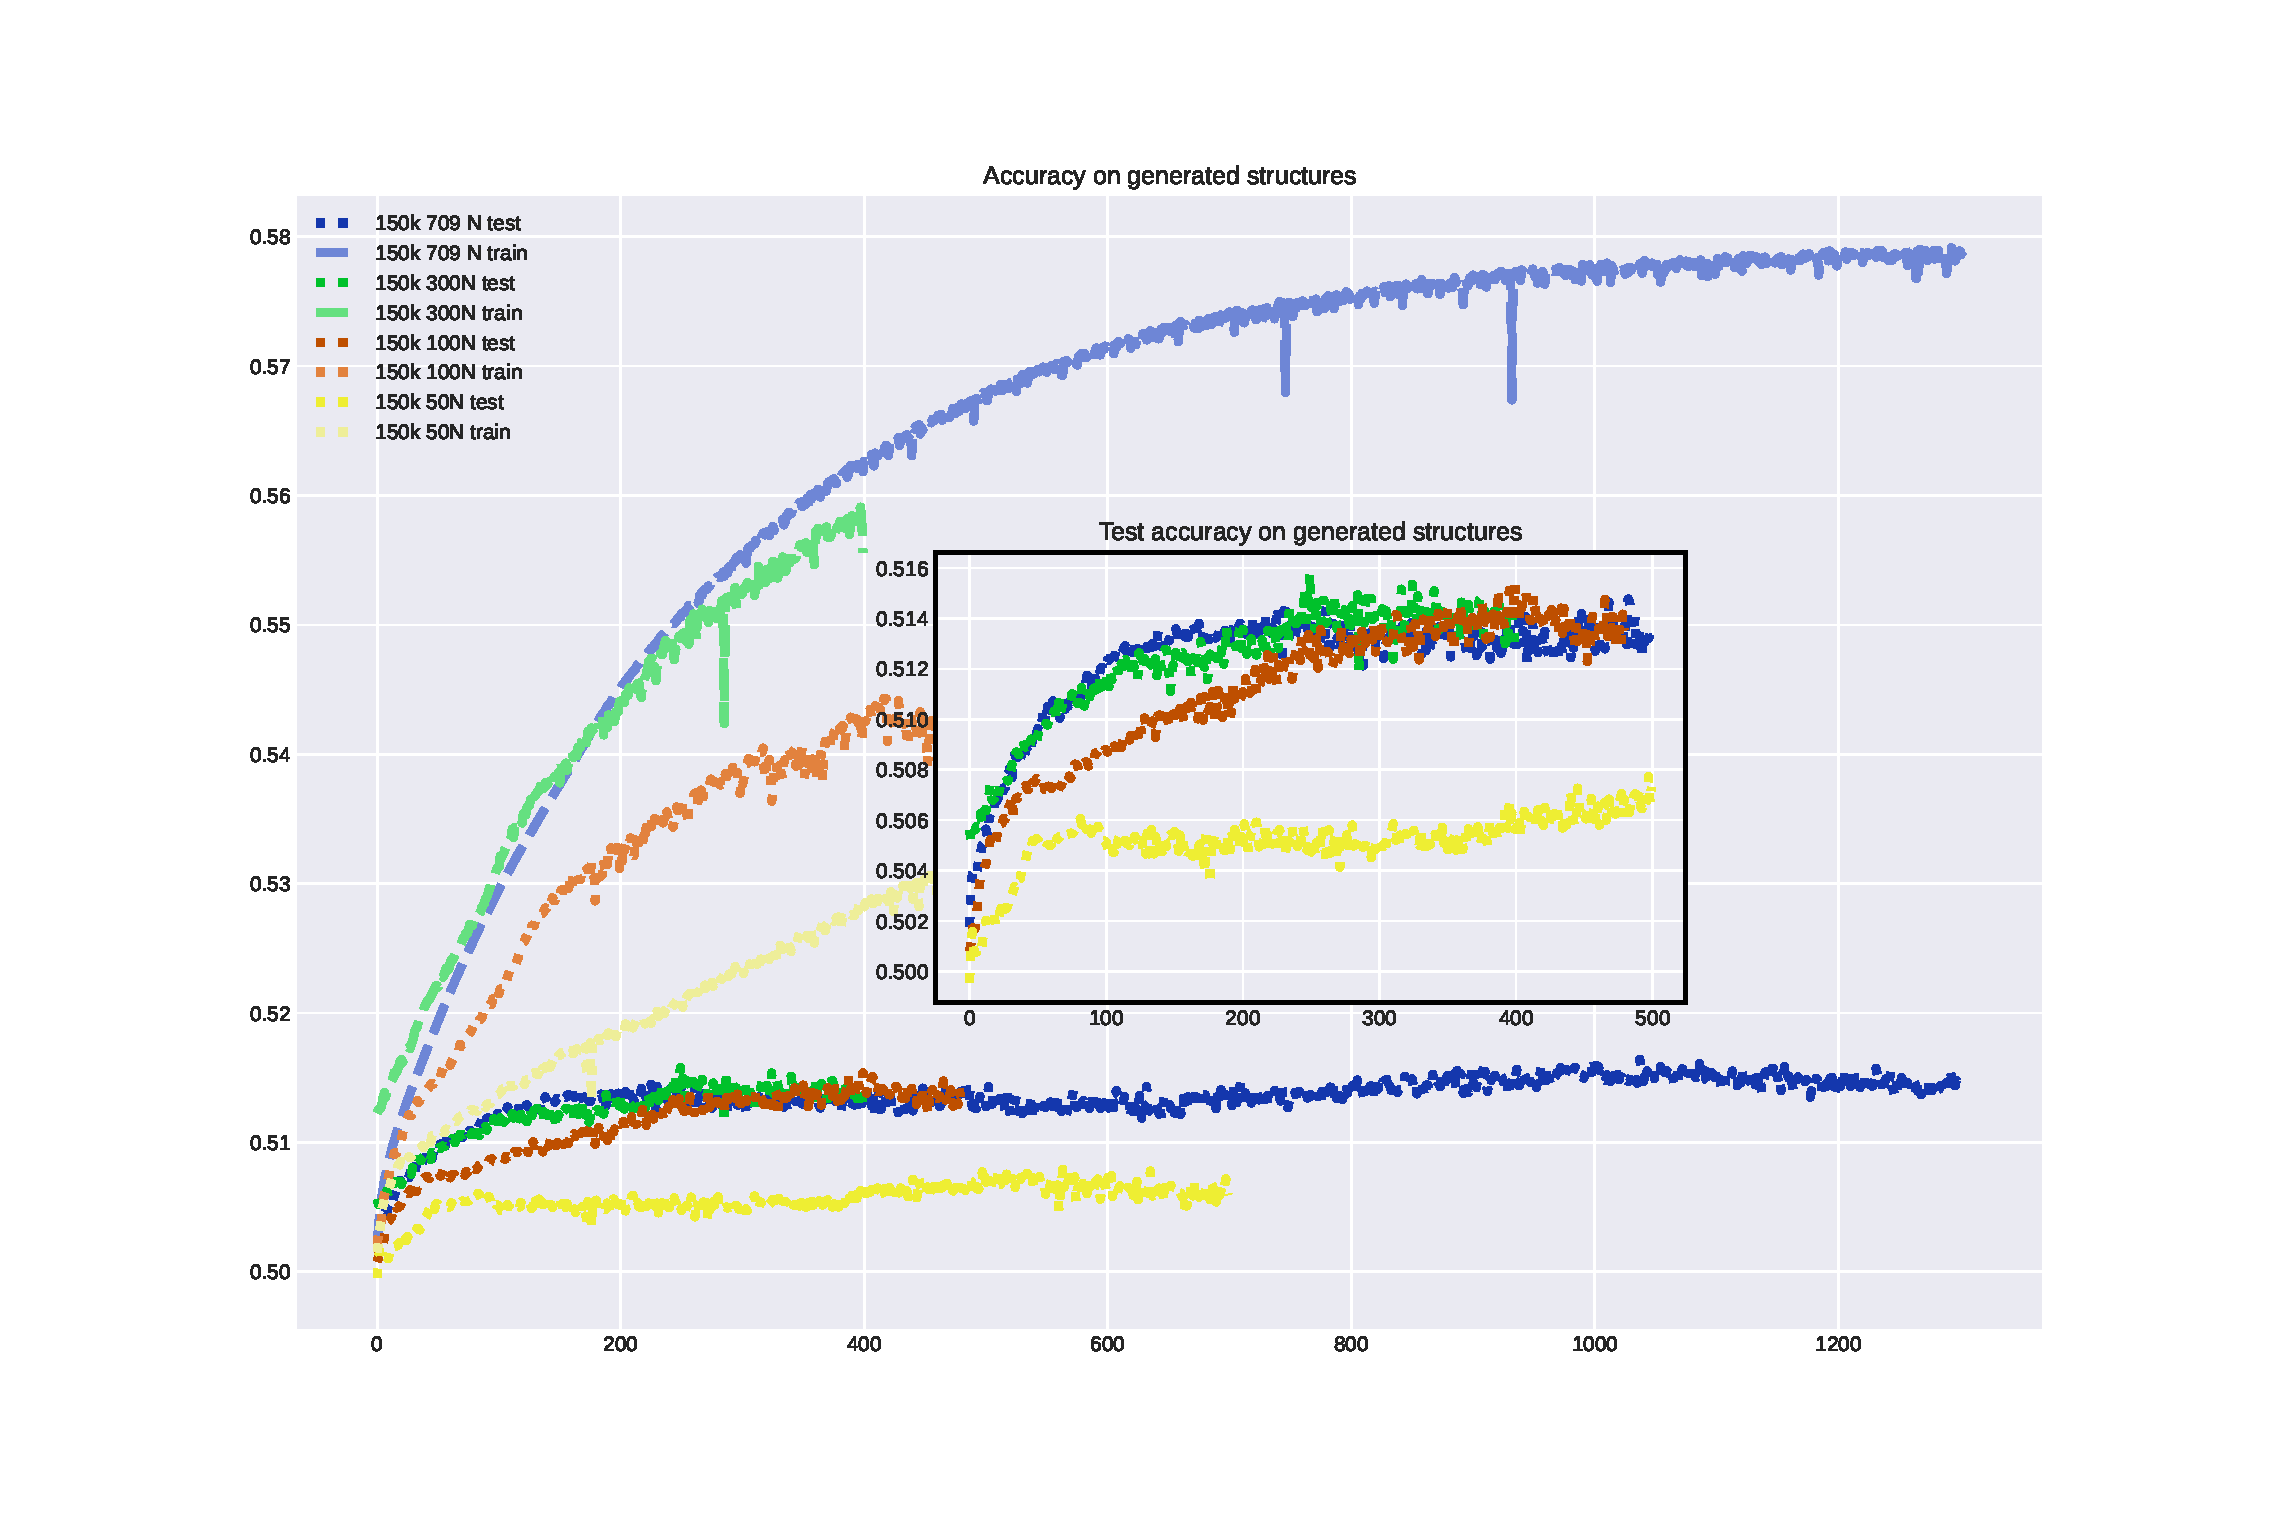
\includegraphics[scale=.500]{imgs/acc-lsize.eps}
\caption{}
\label{}
\end{figure}

\begin{figure}[h!tp]
\centering
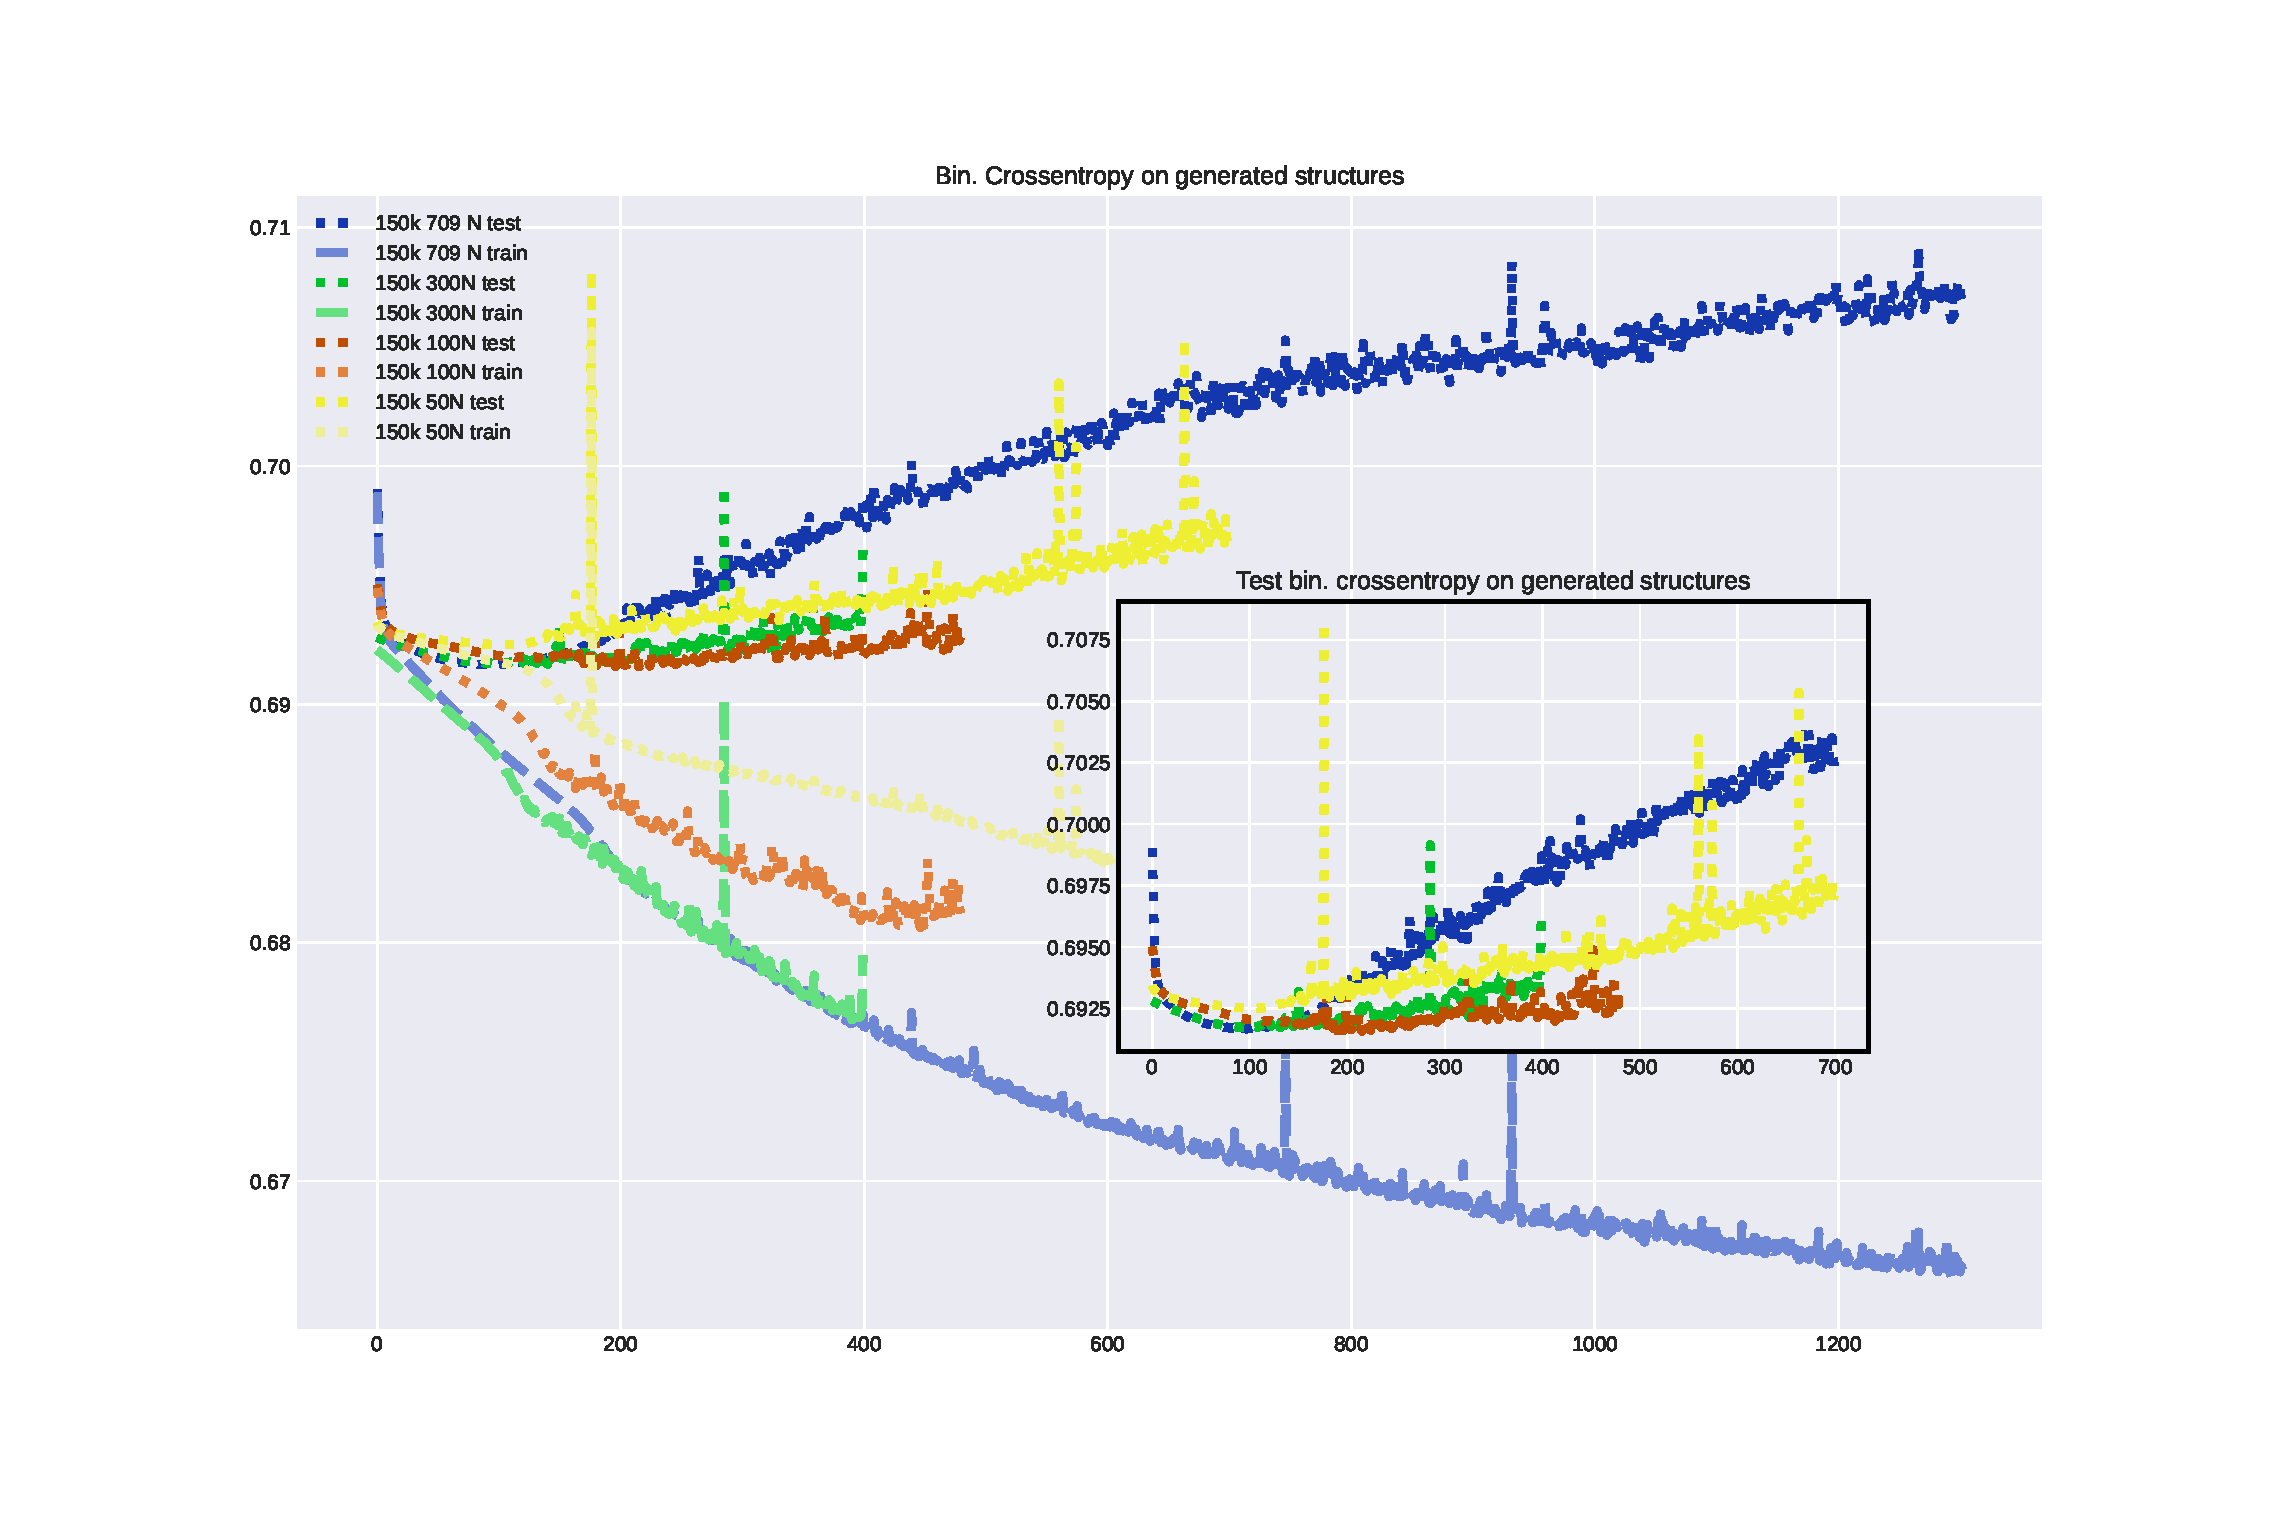
\includegraphics[scale=.500]{imgs/loss-lsize.eps}
\caption{}
\label{}
\end{figure}

\begin{figure}[htp]
\centering
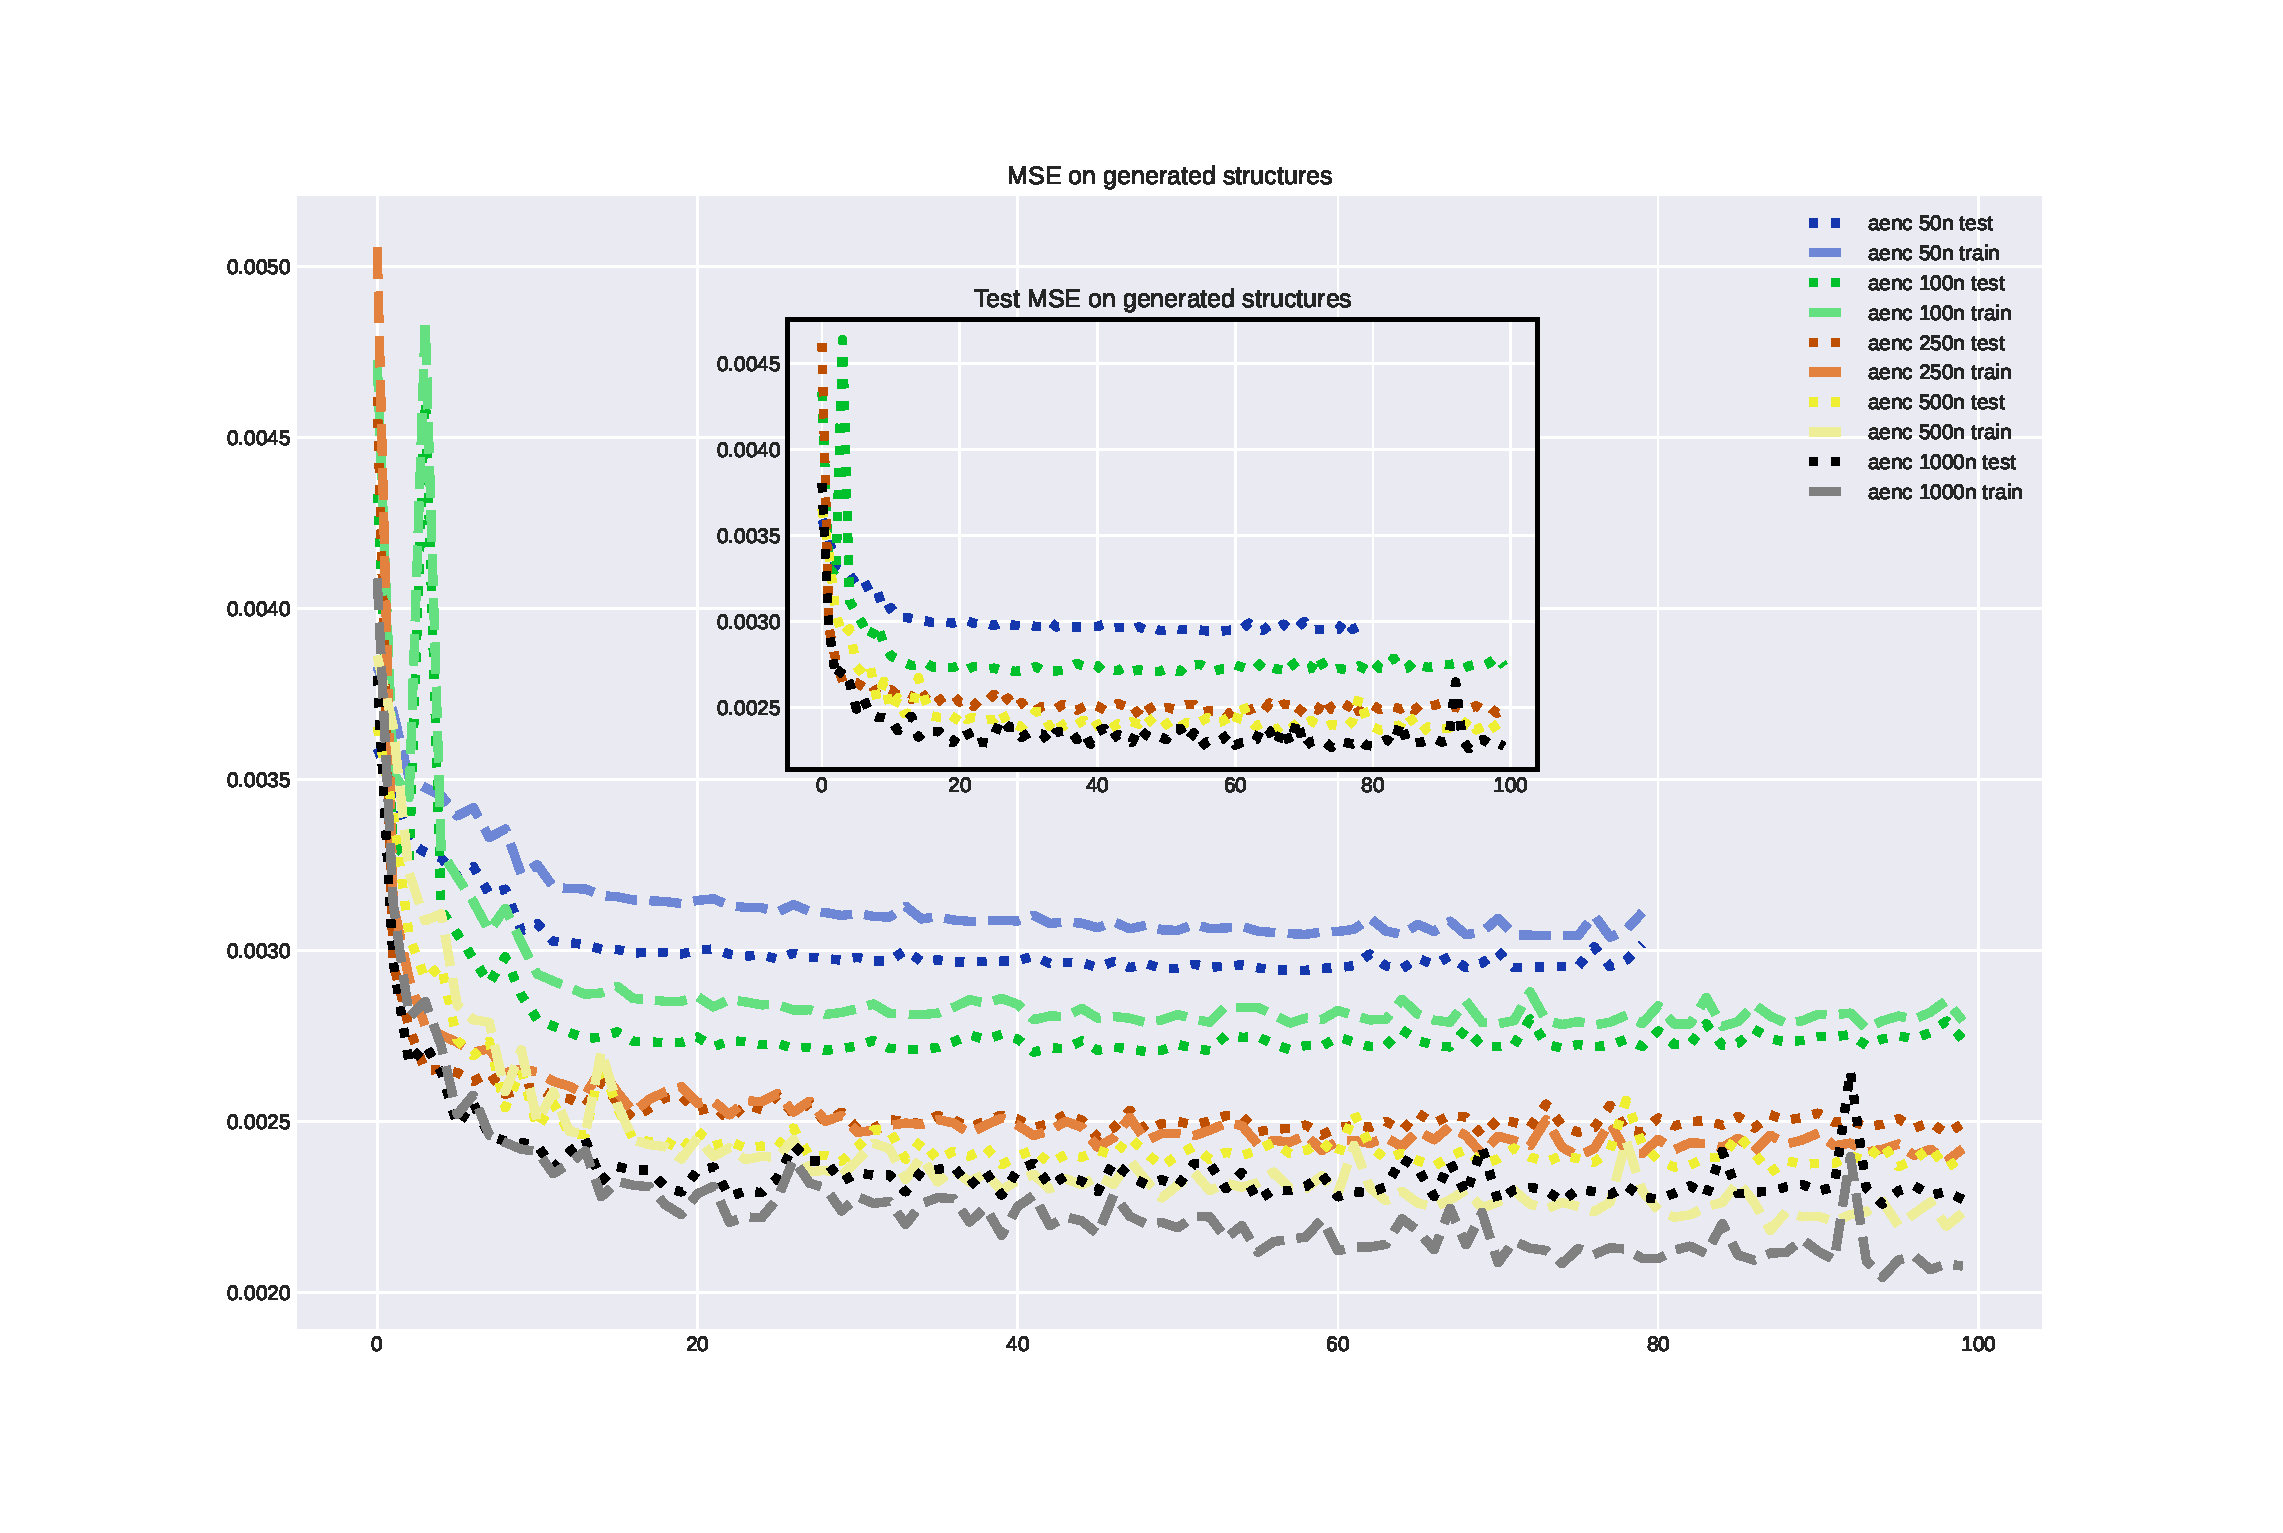
\includegraphics[scale=0.50]{imgs/loss-aenc.eps}
\caption{}
\label{}
\end{figure}

\begin{figure}[htp]
\centering
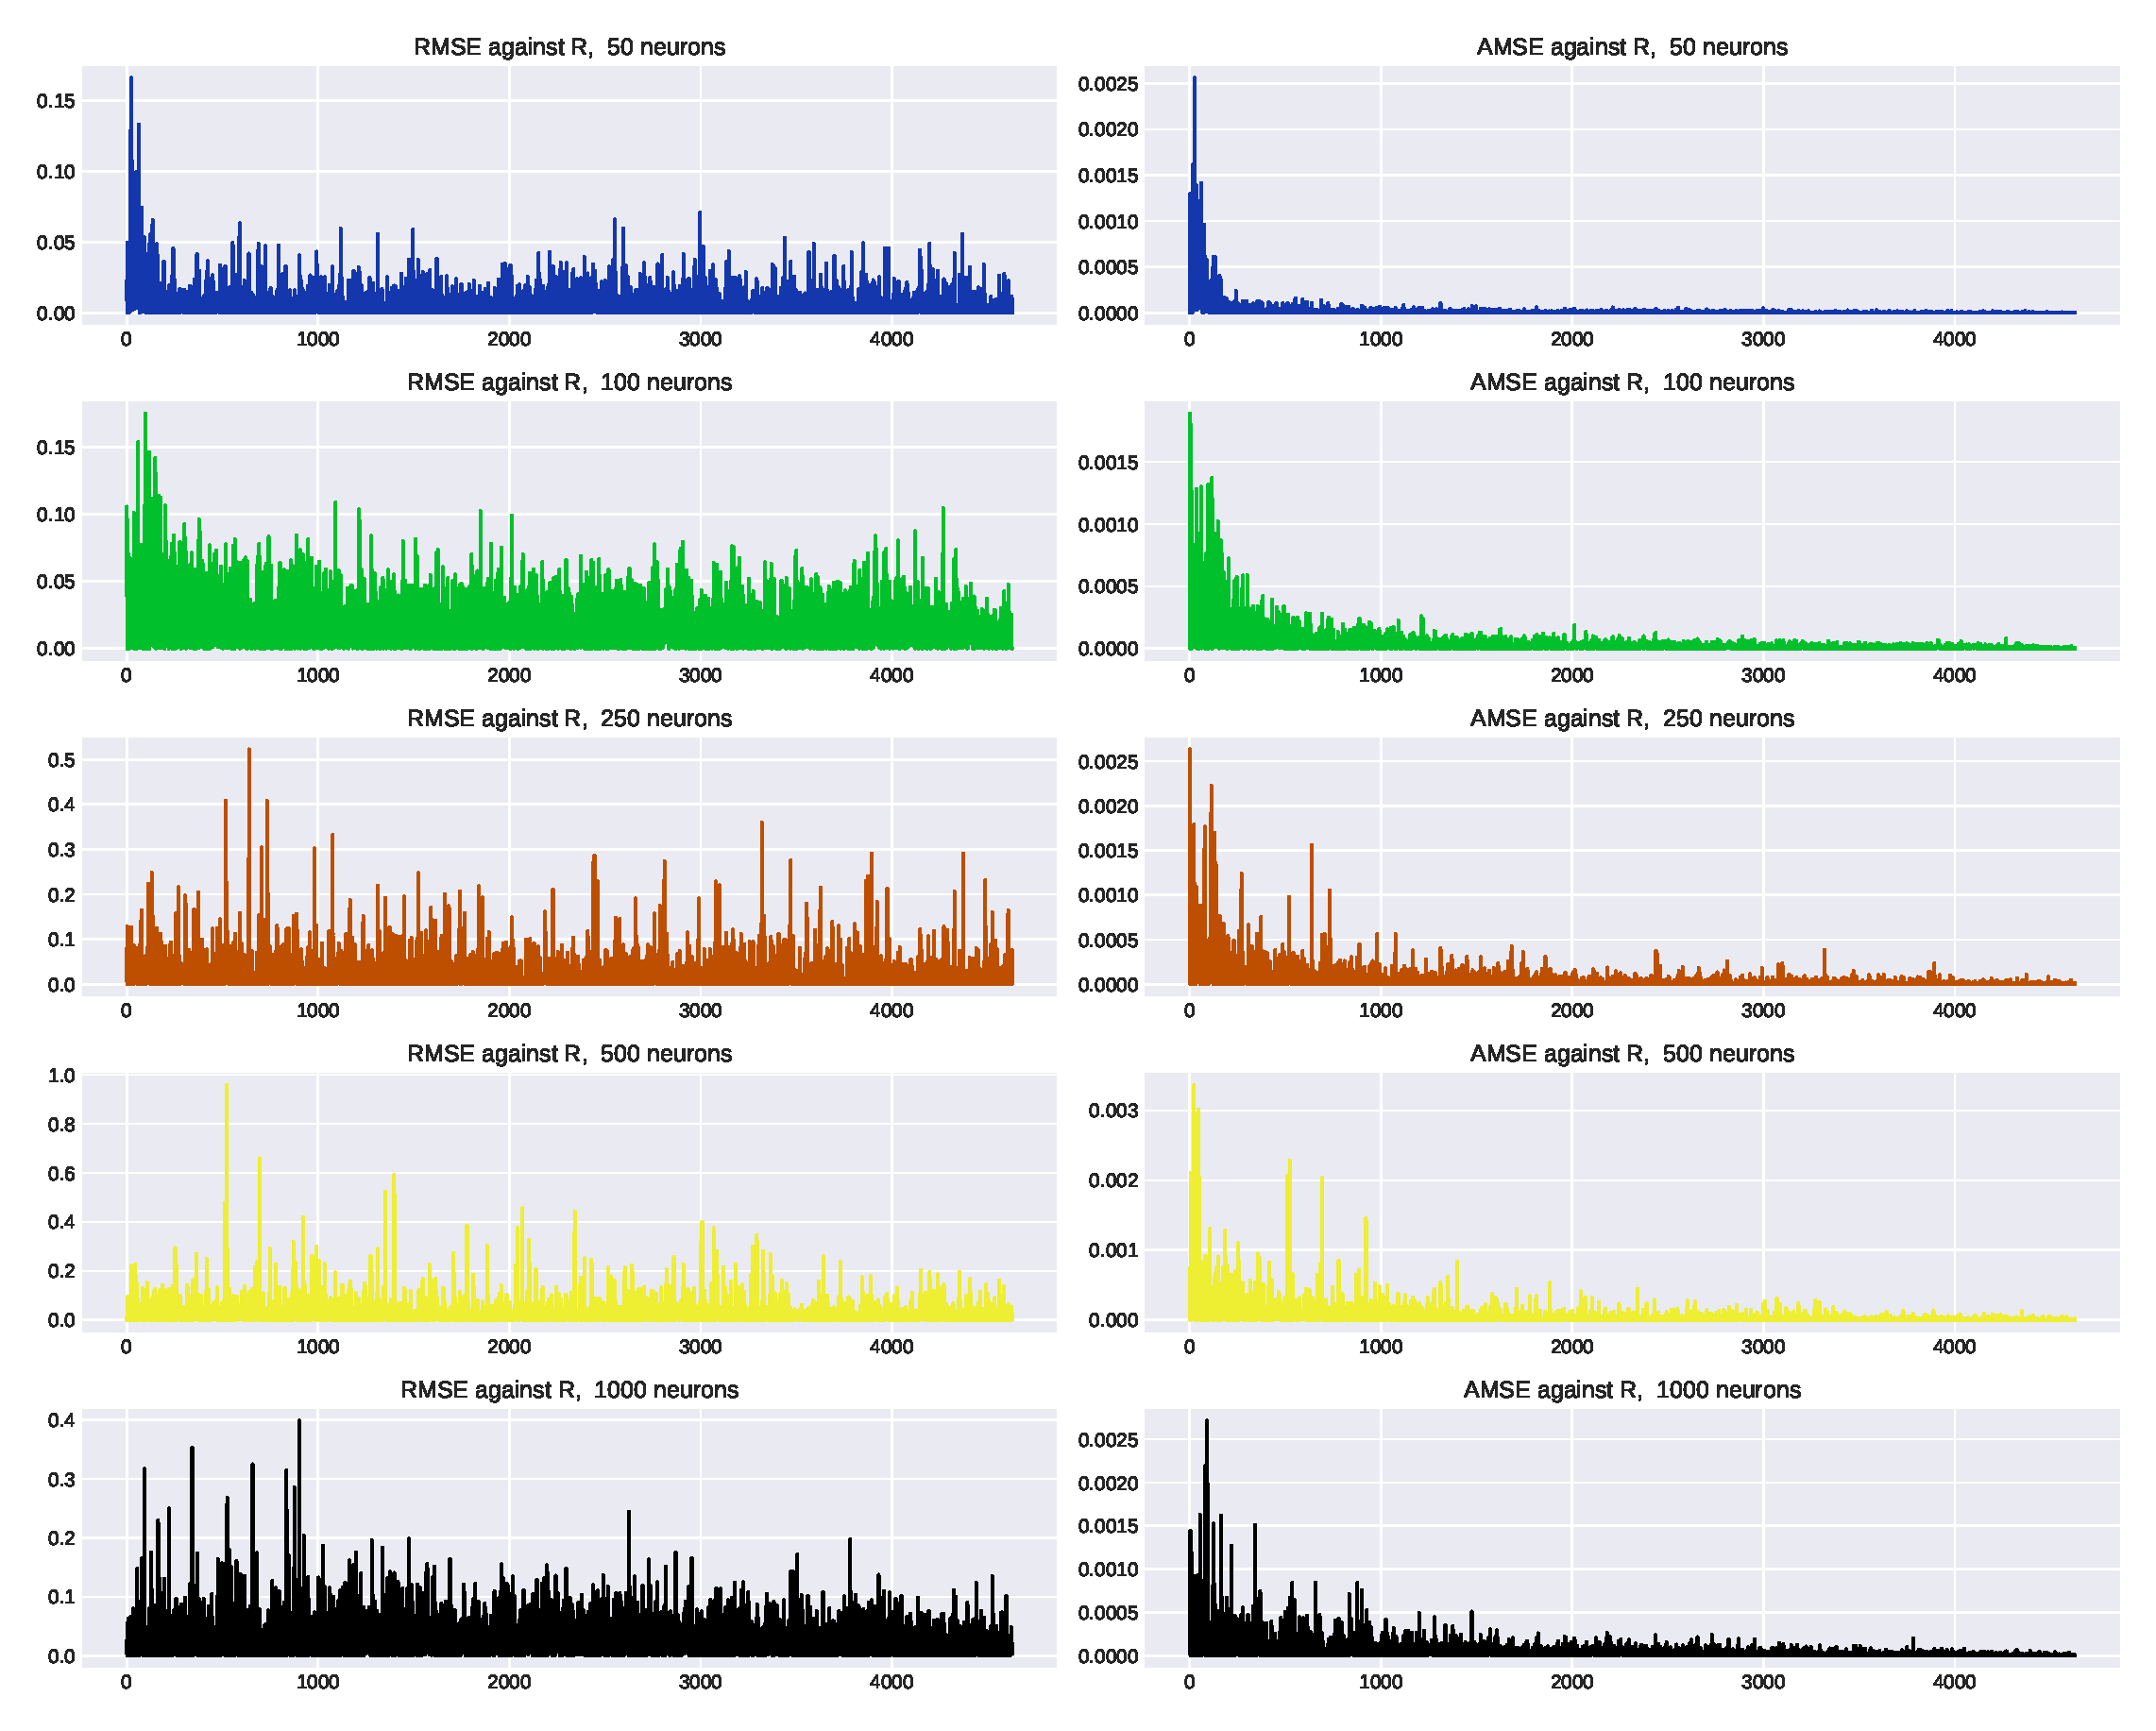
\includegraphics[scale=0.50]{imgs/aenc-errdist.eps}
\caption{}
\label{}
\end{figure}


\begin{figure}[htp]
\centering
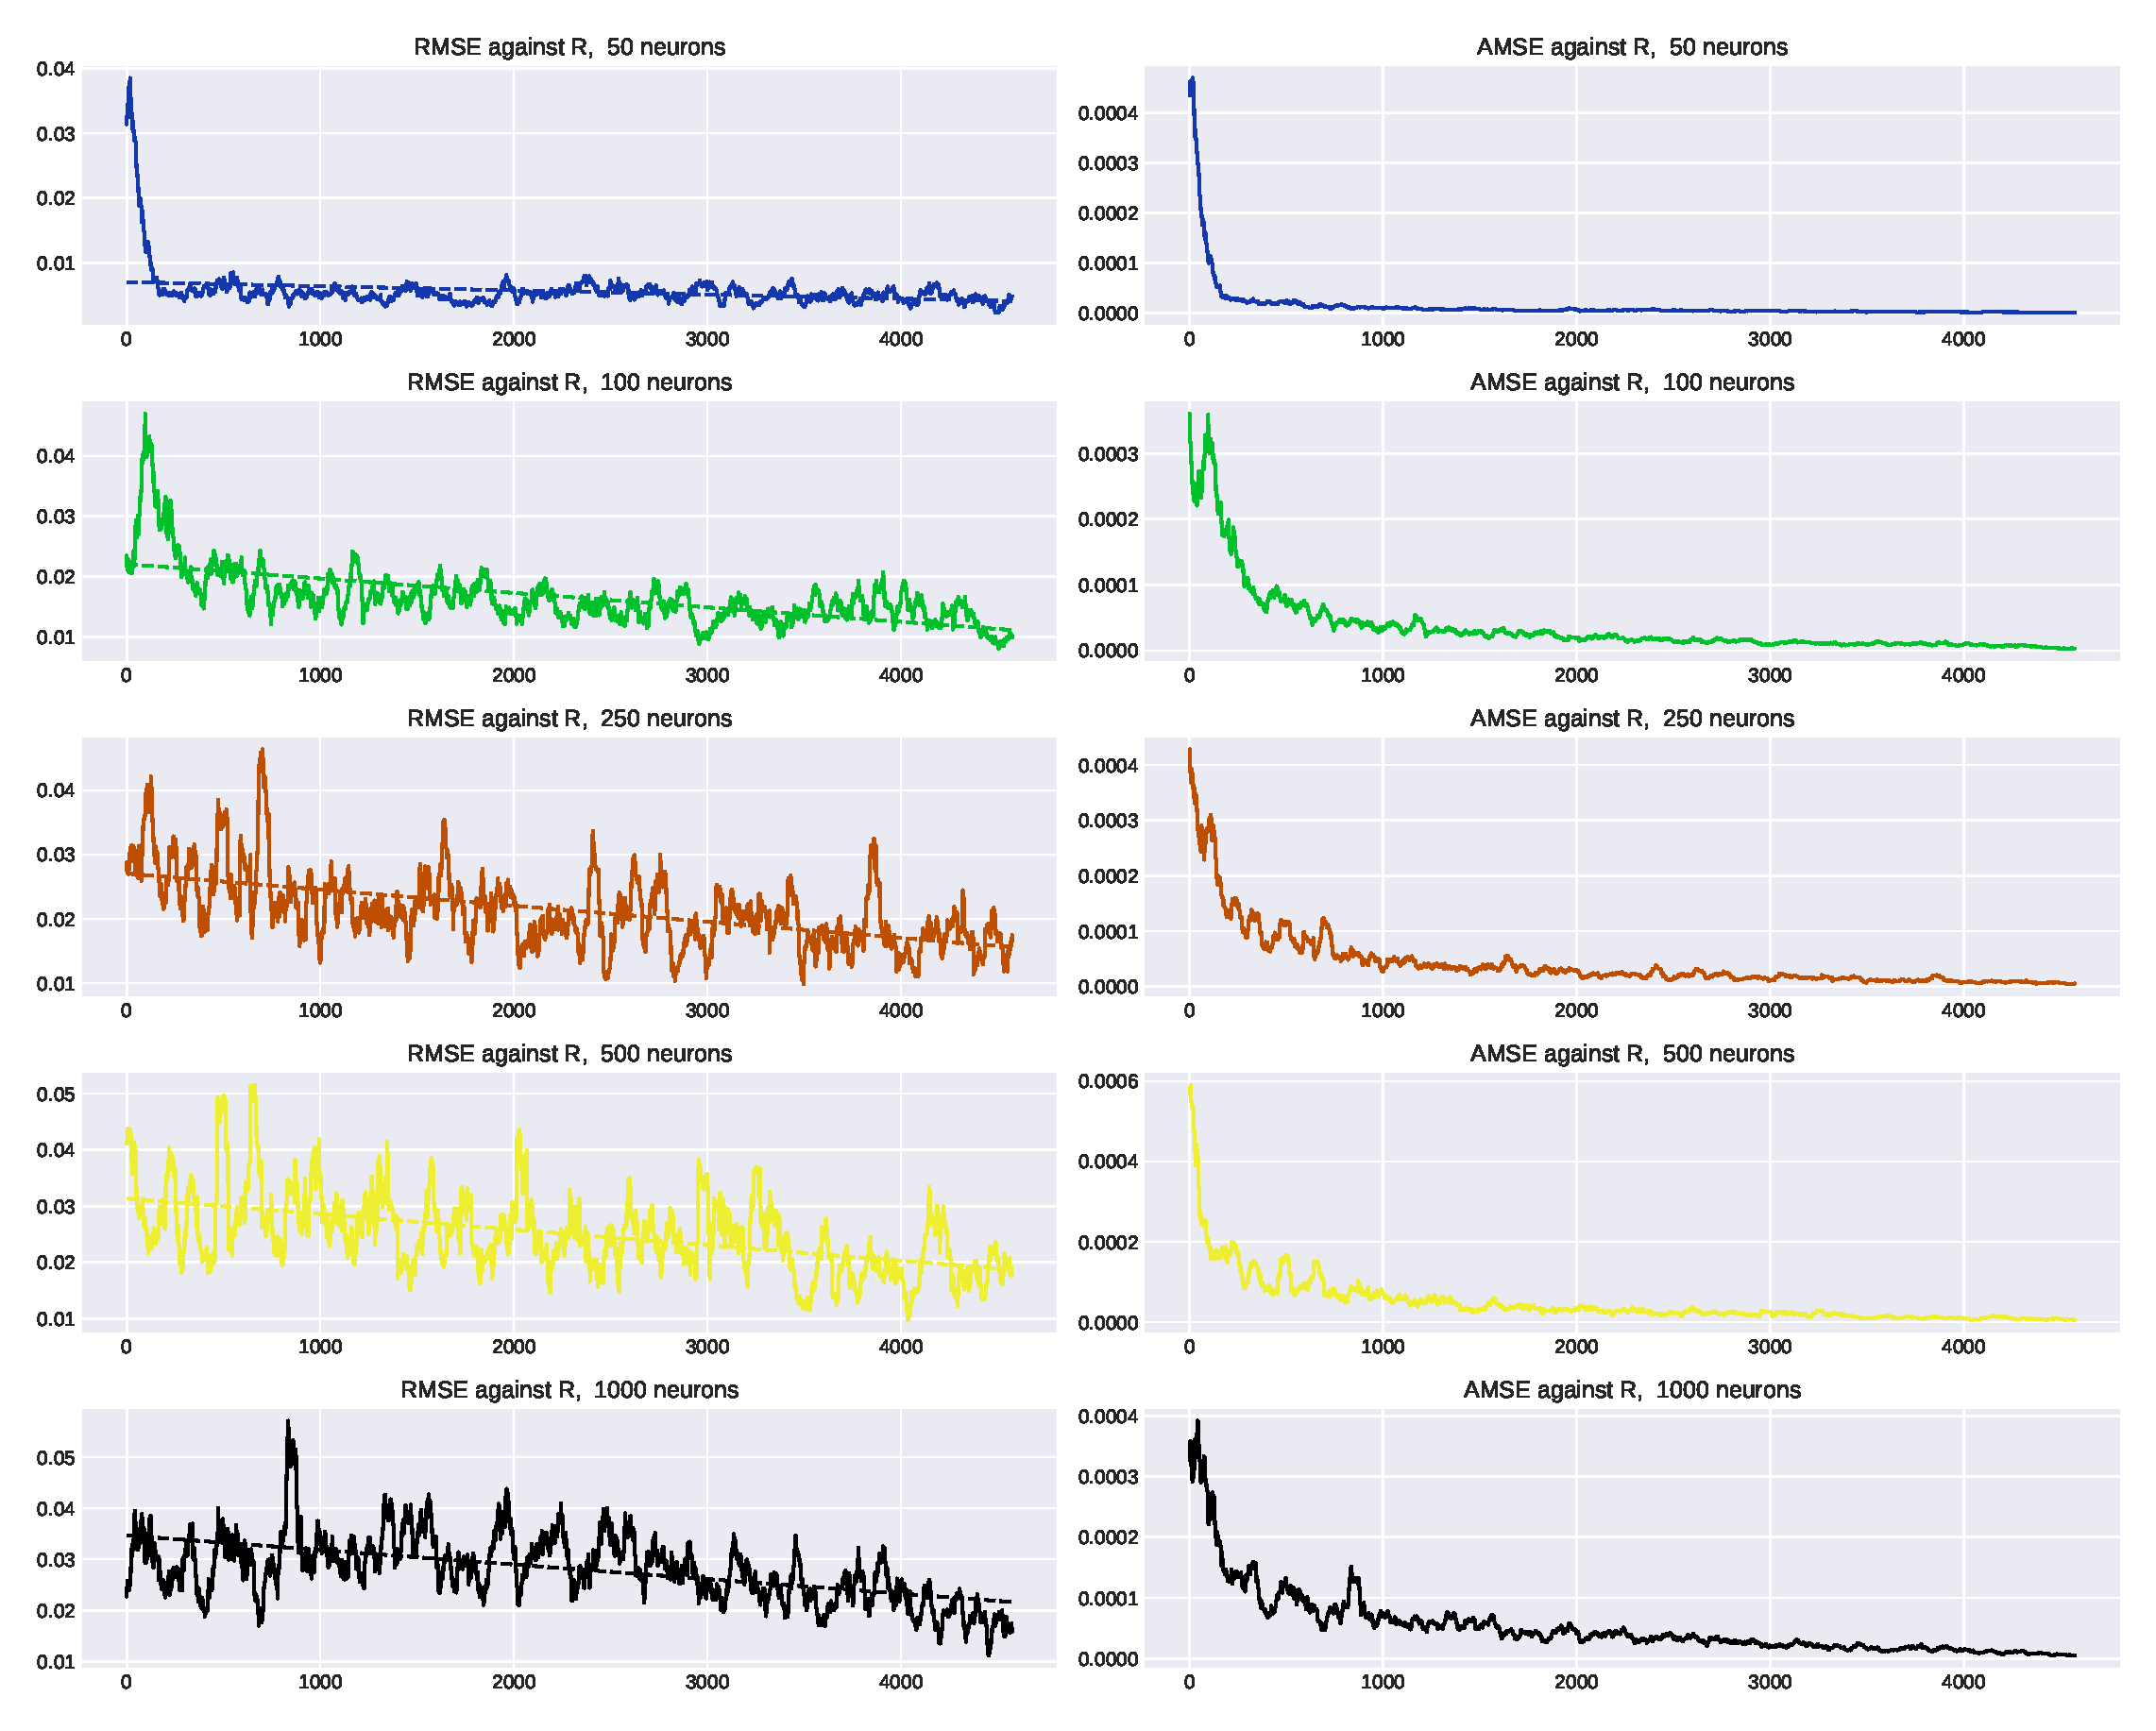
\includegraphics[scale=0.50]{imgs/aenc-errdist_fl.eps}
\caption{}
\label{}
\end{figure}

\section{РЕЗУЛЬТАТЫ И ВЫВОДЫ}



\end{document}
